	\documentclass[twocolumn,
               prd,
               aps,
               superscriptaddress,
               tightenlines,
               nofootinbib,
               eqsecnum,
               amsfonts,
               amsmath,
               longbibliography]{revtex4-1}

\usepackage{epsfig}
\usepackage{graphics}
\usepackage{graphicx}
\usepackage[dvipsnames,table]{xcolor}
\usepackage{bm}
\usepackage{txfonts}
% \usepackage{newtxtext}
% \usepackage{newtxmath}
\usepackage{natbib}
\usepackage{amssymb}
\usepackage{xspace}
\usepackage[normalem]{ulem} % To get strikethrough (\sout)
\usepackage[colorlinks]{hyperref}
\usepackage[caption=false]{subfig}
\usepackage{url}
\usepackage{float}
\usepackage[bottom]{footmisc}
\usepackage{lineno}
\usepackage{mathrsfs}
\usepackage{makecell}
\usepackage{microtype}

% \usepackage{tikz}

% -----------
% Bibligraphy
% -----------
\AtBeginDocument{%
    \newwrite\bibnotes
    \def\bibnotesext{Notes.bib}
    \immediate\openout\bibnotes=\jobname\bibnotesext
    \immediate\write\bibnotes{@CONTROL{REVTEX41Control}}
    \immediate\write\bibnotes{@CONTROL{%
    apsrev41Control,author="08",editor="1",pages="1",title="0",year="1"}}
    \if@filesw
    \immediate\write\@auxout{\string\citation{apsrev41Control}}%
    \fi
}
% -----------

\definecolor{rred}{RGB}{218,41,28}
\hypersetup{linkcolor=NavyBlue}
\hypersetup{citecolor=NavyBlue}
\hypersetup{urlcolor=NavyBlue}

\usepackage{perpage}
\MakePerPage{footnote}

\newcommand{\paperone}{Paper~I\xspace}

\newcommand{\h}{\mathpzc{h}}
\newcommand{\Hhat}{\hat{\mathpzc{H}}}
\newcommand{\B}{\mathpzc{B}}
\newcommand{\hlm}{\mathpzc{h}_{\ell m}}
\newcommand{\xilm}{\xi_{\ell m}}
\newcommand{\Ylm}{{Y}^{-2}_{\ell m}}
\newcommand{\Y}{{Y}^{-2}}
\newcommand{\hc}{h_\times}
\newcommand{\hp}{h_+}
\newcommand{\Fc}{F_\times}
\newcommand{\Fp}{F_+}
\newcommand{\Mf}{M_f}
\newcommand{\cA}{\mathpzc{A}}
\newcommand{\lm}{_{\ell m}}
\newcommand{\deff}{d_\mathrm{eff}}
\newcommand{\rmi}{\mathrm{i}}
\newcommand{\blambda}{\bm{\lambda}}
\newcommand{\btheta}{\bm{\theta}}
\newcommand{\bxi}{\bm{\xi}}
\newcommand{\bxigr}{\bm{\xi}_{\text{GR}}}
\newcommand{\bxingr}{\bm{\xi}_{\text{nGR}}}
\newcommand{\bzeta}{\bm{\zeta}}
\newcommand{\bs}[1]{\bm{\vec{S}_{#1}}}
\newcommand{\Mo}{M_{\odot}}
\newcommand{\FFe}{\mathrm{FF}_\mathrm{eff}}
\newcommand{\FF}{\mathrm{FF}}
\newcommand{\e}{\mathrm{e}}
\newcommand{\rhoopt}{\rho_\mathrm{opt}}
\newcommand{\rhosubopt}{\rho_\mathrm{subopt}}
\newcommand{\fqnm}{f}
\newcommand{\sigmaqnm}{\sigma}
\newcommand{\n}{\mathbf{n}}
\newcommand*{\skymapscale}{0.5}
\newcommand*{\paramestscale}{0.455}
\newcommand{\df}[1]{\delta f_{\text{#1}}}
\newcommand{\dtau}[1]{\delta \tau_{\text{#1}}}
\newcommand{\fngr}[1]{f_{\text{#1}}}
\newcommand{\taungr}[1]{\tau_{\text{#1}}}
\newcommand{\fgr}[1]{f ^{\text{GR}}_{\text{#1}}}
\newcommand{\taugr}[1]{\tau ^{\text{GR}}_{\text{#1}}}
\newcommand{\pSEOB}{\texttt{pSEOBNR}}
\newcommand{\SEOB}{\texttt{SEOBNR}}
\newcommand{\gm}{\mathfrak{m}}
\newcommand{\msun}{~{\rm M}_{\odot}}

% Modified gravity related
\newcommand{\pd}{\partial}
\newcommand{\dd}{{\rm d}}
\newcommand{\ii}{{\rm i}}
\newcommand{\dV}{{\rm d}^{4}x \, \sqrt{-g} \,}

\newcommand{\lame}{\lambda_{\rm e}}
\newcommand{\lamo}{\lambda_{\rm o}}

% Comment commands
\usepackage{xcolor}
\newcommand{\agcomm}[1]{{\textcolor{red}{{[AG: #1]}} }}
\newcommand{\ag}[1]{{\textcolor{Maroon}{{#1}} }}
\newcommand{\hs}[1]{{\textcolor{blue}{{[HS: #1]}} }}
\newcommand{\ab}[1]{{\textcolor{green}{{[AB: #1]}} }}

\newcommand{\AEI}{\affiliation{Max Planck Institute for Gravitational Physics (Albert Einstein Institute), Am M\"uhlenberg 1, Potsdam 14476, Germany}}
\newcommand{\UMD}{\affiliation{Department of Physics, University of Maryland, College Park, Maryland 20742, USA}}

\begin{document}

% HS: temporary title. Feel free to add suggestions
\title{Black-hole ringdown as a probe of higher-curvature gravity theories}

\author{Hector O. Silva}     \AEI
\author{Abhirup Ghosh}       \AEI
\author{Alessandra Buonanno} \AEI \UMD

\date{\today}

%%%%%%%%%%%%%%%%%%%%%%%
\begin{abstract}
% General
% Motivation
% What we do
% Main conclusion
\end{abstract}
%%%%%%%%%%%%%%%%%%%%%%%

\maketitle

% --------------------------------------------------------------------------------- %
\section{Introduction}
\label{sec:intro}
% --------------------------------------------------------------------------------- %

\hs{AB will do this.}

\begin{table}[th]
\begin{tabular}{c | c c}
\hline \hline
Theory & Constraint & This work \\
\hline
EdGB        & $\ell_{\rm GB} \leqslant 1.18$~km~(GW)~\cite{Lyu:2022gdr} & -- \\
dCS         & $\ell_{\rm CS} \leqslant 8.5$~km~(EM+GW)~\cite{Silva:2020acr}  & $\ell_{\rm CS} \leqslant 38.7$~km \\
cubic EFT   & -- & $\ell_{\rm cEFT} \leqslant 38.2$~km \\
quartic EFT & $\ell_{\rm qEFT} \leqslant 150$~km~\cite{Sennett:2019bpc}  & $\ell_{\rm qEFT} \leqslant 51.3$~km \\
\hline \hline
\end{tabular}
\caption{\hs{Mention it in the Introduction later, in a sort of `executive summary'.}}
\label{tab:bound_summary}
\end{table}

% --------------------------------------------------------------------------------- %
\section{Overview of modified gravity theories}
\label{sec:review_theories}
% --------------------------------------------------------------------------------- %

We start by briefly reviewing the modified gravity theories we consider in this
paper, what the current observational constraints are and what we know
about BH QNMs in each of these theories.

\subsection{Einstein-dilaton-Gauss-Bonnet gravity}
\label{sec:review_edgb}

This theory belongs to the class of scalar-Gauss-Bonnet theories, which are
described by the action
%
\begin{equation} \label{eq:action_sgb}
    S_{\rm GB} = \frac{1}{16 \pi}
    \int \dV
    \left[
    R - \tfrac{1}{2}(\nabla \varphi)^2
    + \tfrac{1}{4} \ell^{2}_{\rm GB} f(\varphi) \, \mathcal{G}
    \right]\,,
\end{equation}
%
where $g = \textrm{det} \, g$ is the metric determinant, $R$ is the Ricci
scalar and $\varphi$ is a dynamical scalar field that couples to the
Gauss-Bonnet invariant
%
$\mathcal{G} =
R^{\mu\nu\rho\sigma}R_{\mu\nu\rho\sigma}
- 4 R^{\mu\nu}R_{\mu\nu}
+ R^2$.
%
$R_{\mu\nu\rho\sigma}$ and $R_{\mu\nu}$ are the Riemann and Ricci tensors respectively.
%
By itself, $\int \dV \mathcal{G}$ is a boundary term in four dimensions
and hence does not contribute to the field equations~\cite{Myers:1987yn}.
%
However,  when coupled to $\varphi$, it can contribute to the field equation
through the coupling function $f(\varphi)$. The strength of the coupling is
set by $\ell_{\rm GB}$, with dimensions of length.

Different subclasses of this theory are determined by the function $f(\varphi)$
and can be divided into two classes based on the properties of their BH
solutions.
%
In the first class, the first derivative of the coupling function $f'(\varphi) = \dd f  / \dd \varphi$
is always nonzero and BHs are known to always support scalar hair.
%
This is the case of Einstein-dilaton-Gauss-Bonnet (EdGB) gravity, for which $f(\varphi) = \exp(\varphi)$~\cite{Kanti:1995vq}.
%
% \begin{equation}
% f = \exp(\varphi)\,,
% \end{equation}
%
In the second class, $f'(\varphi) = 0$ can vanish for some constant $\varphi_0$.
%
In this case, the theory admits the same stationary, asymptotically flat BH
solutions as GR and those of scalarized BHs~\cite{Doneva:2017bvd,Silva:2017uqg,Macedo:2019sem,Dima:2020yac,Herdeiro:2020wei,Berti:2020kgk}.
%
Examples include the Gaussian $f(\varphi) \propto \exp(-\varphi^2)$~\cite{Doneva:2017bvd} and
the quadratic $f(\varphi) \propto \varphi^2$~\cite{Silva:2017uqg} coupling functions.
BHs in EdGB gravity have scalar hair, to which we can associate a (monopole) scalar charge $Q$,
related to the asymptotic $r^{-1}$\agcomm{In most of these cases $r$ might be intuitive, but just wanted to leave this comment to remind myself that we never define it explicitly.} fall-off of the scalar field. 
%
This charge is not an independent parameter, and depends on the BH's mass and spin, %~\cite{Berti:2018cxi},
thus being a ``secondary hair''~\cite{Coleman:1991ku,Herdeiro:2015waa}.
%
Since the scalar field is sourced by a curvature scalar, $Q$ is larger (smaller), 
 smaller (larger) the BH mass is.

These properties are not mere theoretical curiosities; they have important observational consequences.
%
First, the presence of the scalar charge implies that when in binaries, BHs can source
scalar dipole radiation (see e.g., Refs.~\cite{Yagi:2011xp,Julie:2019sab,Shiralilou:2020gah,Shiralilou:2021mfl,Julie:2022huo})
which affects the GW phase at $-1$PN order (relative to the dominant GR
contribution), with magnitude proportional to the difference between the
charges of binary components. This makes EdGB gravity testable with present GW
observations of compact binaries where at least one component is a BH.
%
More specifically, Ref.~\cite{Lyu:2022gdr} placed the bound
%
$\ell_{\rm GB} \leqslant 1.33$~km
%
using the neutron star-black hole binaries GW200105 and
GW200115~\cite{LIGOScientific:2021qlt} while Refs.~\cite{Nair:2019iur,Perkins:2021mhb}, obtained
%
$\ell_{\rm GB} \leqslant 1.7$~km,
%
by stacking the posteriors of $\ell_{\rm GB}$ from a selection of black hole binaries (BBH)
from the GWTC-1 and GWTC-2 catalogs~\cite{LIGOScientific:2018mvr,LIGOScientific:2020ibl}\footnote{These bounds
are, strictly speaking, valid only when the scalar field $\varphi$ is small, i.e., $\varphi \ll 1$, and
take into account only the leading-order scalar field contribution arising from the dilatonic coupling.}.
Secondly, the scalar field does influence the response of BHs to linearized perturbations and thus
affects the BH QNM spectra.
%
The coupling between scalar field and the Gauss-Bonnet invariant, which
result in a coupling between scalar perturbations and gravitational
perturbations of polar parity can, for example break the equivalence
between the QNM spectra of polar and axial gravitational perturbations
(isospectrality~\cite{Chandrasekhar:1985kt}, see also Refs.~\cite{Glampedakis:2017rar,Lenzi:2021njy}) for Schwarzschild BHs in GR.
%

The QNMs for nonrotating BHs in EdGB gravity were first computed in
Refs.~\cite{Pani:2009wy,Blazquez-Salcedo:2016enn} and were
extended to leading-order in BH spin in Ref.~\cite{Pierini:2021jxd}.

\subsection{Dynamical Chern-Simons gravity}
\label{sec:review_dcs}

This theory is described by the action~\cite{Jackiw:2003pm,Alexander:2009tp},
%
\begin{equation} \label{eq:action_dcs}
    S_{\rm CS} = \frac{1}{16 \pi}
    \int \dV
    \left[
    R - \tfrac{1}{2}(\nabla \vartheta)^2
    + \tfrac{1}{4} \ell^{2}_{\rm CS} \, \vartheta \, {}^{*}RR
    \right],
\end{equation}
%
where $\vartheta$ is a pseudoscalar field which couples to the Pontryagin
density
${}^{*}RR = {}^{*}R_{\mu\nu}{}^{\rho\sigma} R^{\nu\mu}{}_{\rho\sigma}$,
%
where ${}^{*}R^{\mu\nu\rho\sigma}$ is the dual of the Riemann tensor
defined as
%
${}^{*}R^{\mu\nu\rho\sigma} =
\epsilon^{\mu\nu}{}_{\gamma\delta}
R^{\gamma\delta\rho\sigma} / 2$,
%
and $\epsilon_{\mu\nu\gamma\delta}$ is the Levi-Civita tensor.
%
As in scalar-Gauss-Bonnet theories, $\int \dV {}^{*}RR$ by itself is a boundary
term~\cite{Jackiw:2003pm} that does not contribute to the field equations in
four-dimensions.
%
However, a coupling with $\vartheta$ can modify the field equations.
%
The coupling strength is set by the coupling constant $\ell_{\rm CS}$, with
dimensions of length.

The theory admits as a solution, the garden-variety Schwarzschild BH of GR. This
is not the case when rotation is included and the Kerr metric is not a solution of
the theory~\cite{Jackiw:2003pm}.
%
These rotating BHs support a scalar field which fall off as
$r^{-2}$ asymptically, to which we can associate a scalar dipole
charge~\cite{Yunes:2009hc,Konno:2009kg}.
%
As a consequence, the leading-scalar radiative channel of BBH to lose energy is quadrupolar,
which affects the GW phase at 2PN order~\cite{Yagi:2011xp,Alexander:2017jmt}.\agcomm{I am not sure I understand this sentence.}
%
Deviations from GR at this PN order are poorly constrained with present GW
observations~\cite{LIGOScientific:2021sio}\agcomm{might want to quantify what we mean by poor. Looking at Table VI of the reference, I see that the 90\% credible bounds are $\sim 1-0\%$ using the hierarchical approach and $\sim 50\%$ using the restricted approach for $\varphi_4$. Perhaps we want to mention this?}, making dCS gravity unconstrained by
analyses that rely on the inspiral portion of GWs from BBH
binaries~\cite{Nair:2019iur,Perkins:2021mhb}.
%
Nonetheless, the theory has been constrained in Ref.~\cite{Silva:2020acr}, that found
%
$\ell_{\rm CS} \leqslant 8.5$~km,
%
by folding data from the X-ray observations of the isolated neutron star (NS)
PSR~J0030+0451~\cite{Lommen:2000yt,NANOGrav:2017wvv} by
NICER~\cite{Riley:2019yda,Miller:2019cac} and from the GW observation of the binary
neutron star (BNS) GW170817~\cite{TheLIGOScientific:2017qsa,LIGOScientific:2018cki}.

The QNMs of the Schwarzschild BH in dCS gravity were studied in
Refs.~\cite{Yunes:2007ss,Cardoso:2009pk,Molina:2010fb}, that found that scalar
perturbations couple to gravitational perturbations of axial parity. (Contrast
with EdGB gravity)\agcomm{Is the text in parenthesis a comment?}.
%
This leads to a breakdown of isospectrality. The QNM spectra of slowly-rotating BHs in dCS gravity was
studied in Ref.~\cite{Wagle:2021tam}.
%
They were also extracted from numerical relativity (NR) simulations of head-on BH collisions
in Ref.~\cite{Okounkova:2019dfo}.

\subsection{Effective-field-theory of GR}

Our last example of modified gravity theories are the so-called effective field
theories (EFT) of GR~\cite{Endlich:2017tqa,Sennett:2019bpc,deRham:2020ejn,Cano:2020cao,Cano:2021myl}.
%
They are described by the action
%
\begin{equation} \label{eq:action_eft}
    S_{\rm EFT} = \frac{1}{16 \pi}
    \int \dd^4x \sqrt{-g}
    \left[ R
    +
    \sum_{n \geqslant 2} \ell^{2n - 2} L^{(2n)}
    \right]\,,
\end{equation}
%
where $\ell$ is a length-scale assumed to be small compared to the length-scale
$\ell / M \ll 1$ associated with a BH and $L^{(2n)}$ are corrections 
that introduce higher-order curvature tensors (with $2n$ metric derivatives).

More specifically, we follow the notation of
Refs.~\cite{Cano:2020cao,Cano:2021myl} and work up to dimension-eight operators
($n=4$),
%
\begin{subequations}
\label{eq:action_mods}
\begin{align}
    L^{(6)} &= \lame R_{\mu\nu}{}^{\rho\sigma} R_{\rho\sigma}{}^{\gamma\delta} R_{\gamma \delta}{}^{\mu\nu}
    + \lamo R_{\mu\nu}{}^{\rho\sigma} R_{\rho\sigma}{}^{\gamma\delta} \tilde{R}_{\gamma \delta}{}^{\mu\nu}\,,
    \label{eq:s_6}
    \\
    L^{(8)} &= \varepsilon_{1} \mathcal{C}^2
    + \varepsilon_{2} \tilde{\mathcal{C}}^{2}
    + \varepsilon_{3} \mathcal{C} \tilde{\mathcal{C}}\,,
\label{eq:s_8}
\end{align}
\end{subequations}
%
where ${\cal C} = R_{\mu\nu\rho\sigma} R^{\mu\nu\rho\sigma}$,
$\tilde{\cal C} = R_{\mu\nu\gamma\delta} \epsilon^{\mu\nu}{}_{\rho\sigma} R^{\rho\sigma\gamma\delta}$,
and $(\lambda_{\rm o, e},\varepsilon_{i})$,  $i=1,2,3$, are dimensionless parameters.
%
Due to the large number of free parameters in this theory, we will focus on a subset of the parameter space.
%
In particular, we will consider dimension-six and dimension-eight operators separately.
%
In the dimension-six case we further assume that $\lame = \lamo = 1$, leaving us with $\ell = \ell_{\rm cEFT}$
as our single free parameter.
%
In the dimension-eight case, we will set $\varepsilon_{1} = 1$ and $\varepsilon_{2} = \varepsilon_{3} = 0$,
as done in Ref.~\cite{Sennett:2019bpc}.
%
This leaves us with $\ell = \ell_{\rm qEFT}$ as our single free parameter \agcomm{Perhaps a bit of motivation about why we make these choices, even if it is to say that it is a simple first choice?}.

In general \dots
%
\hs{Alessandra, can you include a short description of~\cite{Sennett:2019bpc} for the quartic EFT?}

The QNMs of nonrotating BHs where calculated in Refs.~\cite{deRham:2020ejn,Cano:2020cao} in the dimension-six EFT
and in Refs.~\cite{Cardoso:2018ptl,Cano:2020cao} in the dimension-eight EFT.
%
Ref.~\cite{Cano:2020cao} calculated the leading-order BH spin corrections to the QNM spectra.

% --------------------------------------------------------------------------------- %
\section{Methods}
\label{sec:method}
% --------------------------------------------------------------------------------- %

Having reviewed the modified gravity theories we will consider, we now present
the sequential building blocks for the waveform model we use to test these theories
against GW observations.
%
We start by reviewing the theory-agnostic parametrized ringdown
spin-expansion coefficients (ParSpec) \sout{expansion} \ag{framework} \agcomm{replaced `framework' to prevent duplication.  The original parspec authors call this a data-analysis framework, so I think it would be safe to use it. I have left the term ``ParSpec expansion" in other places, because ParSpec is always abbreviated in those places.} in Sec.~\ref{sec:review_parspec}.
%
Next, in Sec.~\ref{sec:review_pSEOB}, we review our baseline
parametrized inspiral-(plunge)-merger-ringdown (IMR) BBH waveform
model~\cite{Brito:2018rfr,Ghosh:2021mrv} and explain how we modify
it to include the ParSpec expansion.
%
Finally, in Sec.~\ref{sec:theory_specific_qnm}, we show how we can map
theory-specific QNM calculations in modified gravity theories onto the
theory-agnostic free coefficients in the ParSpec expansion.
%
Ultimately, this provides us with an IMR BBH waveform model, with the ringdown
portion of the model informed by QNM calculations in specific beyond-GR
theories.

\subsection{The parametrized ringdown spin expansion coefficients framework}
\label{sec:review_parspec}

We start by reviewing the ParSpec
framework introduced in Ref.~\cite{Maselli:2019mjd}, but following
some of the notation used in Ref.~\cite{Carullo:2021dui}.
%
A general procedure to describe deviations to the QNM frequencies $\omega_{k}^{\rm Kerr}$ and
damping times $\tau_{k}^{\rm Kerr}$ of the GR Kerr BH is to write,
%
\begin{subequations}
\label{eq:general_deviation}
\begin{align}
\omega_{k} &= \omega^{\rm Kerr}_{k} \, (1 + \delta \omega_{k}), \\
\tau_{k}   &= \tau^{\rm Kerr}_{k}   \, (1 + \delta \tau_{k}),
\end{align}
\end{subequations}
%
where $\delta\omega_{k}$ and $\delta\tau_{k}$ are the fractional deformation parameters.
%
Here we use the subscript $k$ to represent the QNM labels $\{l,\, m,\, n\}$,
where $l$ and $m$ are the multipole indices, and $n$ the overtone number.
%
This type of parametrization was adopted, for instance, in Refs.~\cite{Gossan:2011ha,Meidam:2014jpa,Carullo:2018sfu}.

\ag{The current LIGO-Virgo-Kagra tests of BH ringdown (see Sec.VII.A of~\cite{LIGOScientific:2020tif} or Sec.VIII.A of~\cite{LIGOScientific:2021sio}) take a restrictive theory-agnostic approach towards the inference of $\delta\omega_{k}$ and $\delta\tau_{k}$. These deviations are either assumed to occur identically across all observed sources or belong to a generic underlying Gaussian population. A more realistic scenario, however, is that these parameters depend on the source BH's mass and spin.}
\sout{A caveat of parametrizations of the form~\eqref{eq:general_deviation}, is that
$\delta\omega_{k}$ and $\delta\tau_{k}$ depend, in general, on the BH's source mass and spin.}
%
Ideally, one would like to explicitly reinstate \sout{the dependence the source-frame
BH mass and spin} \ag{this dependence} for it would
%
(i) introduce deformation parameters which can be determined, once and for
all, from a specific gravity theory (GR included), and
%
(ii) make it simpler to combine constraints coming from multiple \ag{(independently observed)} sources.

ParSpec is such an observable-based
\sout{In the ParSpec expansion this is accomplished by performing a} bivariate
expansion of Eq.~\eqref{eq:general_deviation} in the detector-frame BH's mass
$M$ and spin $\chi$, \sout{namely}
%
\begin{subequations}
\label{eq:kerr_expansion}
\begin{align}
\omega_{k} &= \frac{1}{M} \sum_{n = 0}^{N_{\rm max}} \, \chi^{n} \omega^{(n)}_{k} \, \left( 1 + \gamma \delta \omega^{(n)}_{k} \right), \\
\tau_{k}   &= M     \sum_{n = 0}^{N_{\rm max}} \, \chi^{n} \tau^{(n)}_{k}   \, \left( 1 + \gamma \delta \tau^{(n)}_{k} \right),
\end{align}
\end{subequations}
%
where $\omega_{k}^{(n)}$ and $\tau_{k}^{(n)}$ are dimensionless coefficients of the
expansion in spin for Kerr QNMs\footnote{\ag{From this point onwards, to prevent ambiguity,
we will use $n$ to denote the series expansion index, and not the spherical 
harmonic overtone.}};
%
$\delta\omega_{k}^{(n)}$ and $\delta\tau_{k}^{(n)}$ are source-independent
dimensionless coefficients that characterize the corrections to the Kerr QNM at
each spin-order;
%
and $N_{\rm max}$ is the order of the spin expansion.
%
All source dependence on a given modified gravity theory is contained in the
dimensionless parameter $\gamma$, given by
%
\begin{equation}
\gamma
%
= \left(\frac{\ell}{M_{\rm s}}\right)^{p}
%
= \left[
\frac{\ell c^2 (1 + z)}{G M}
\right]^{p},
\label{eq:def_gamma}
\end{equation}
%
which depends on a parameter $\ell$, with dimensions of length (and sets the
length-scale at which beyond-GR modifications become important), and
the exponent $p$ which is related to how the beyond-GR modifications are
added to the Einstein-Hilbert action.
%
In Eq.~\eqref{eq:def_gamma} we made \sout{$\ell$} \ag{$\gamma$} dimensionless  by using the other
length-scale associated with the remnant black hole, i.e., its source-frame mass
$M_{\rm s}$\footnote{\ag{Throughout this paper, we maintain the convention of 
using the subscript ``s" to denote source-frame quantities and plain baseline 
symbols for detector-frame measurements.}} which we can also write in terms of the detector-frame mass $M$ through
the redshift $z$~\cite{Krolak:1987ofj}. \ag{Also, dividing by the factor $G/c^2$ allows us to
express $\ell$ in physically intuitive metric units.}

In principle, a modification to GR would also affect $M$ and $\chi$ and the
expansion should be written in terms of the non-GR mass and spin, say $\bar{M}$ and
$\bar{\chi}$. If we assume that the beyond-GR corrections are included perturbatively
(as is the case of all theories described in Sec.~\ref{sec:review_theories}),
the modifications to the BH mass and spin can be absorbed into the deviations
parameters $\delta\omega$ and $\delta\tau$.
%
This means we can identify the $M$ and $\chi$ with their \emph{corresponding GR values}
\footnote{\ag{For a more detailed discussion, see Appendix A in ~\cite{Maselli:2019mjd}.}}.
%
We will see that in Sec.~\ref{sec:pe} that this assumption is indeed
satisfied in our parameter estimation studies (cf.~Fig.~\ref{fig:corner_plot}).

Finally, we remark that in the GR limit ($\gamma \to 0$)
the series~\eqref{eq:kerr_expansion} truncated at $N_{\rm max} = 4$, reproduces with 1\% accuracy
the Kerr QNMs for spins $\chi \lesssim 0.7$.
%
The values of the fitting coefficients $\omega_{k}^{(n)}$ and $\tau_{k}^{(n)}$
can be found in Ref.~\cite{Maselli:2019mjd}, Table I\agcomm{This sentence would need
to be adapted if we put the GR coefficients in our current Table II.}.
%
In Ref.~\cite{Carullo:2021dui}, the fitting coefficients were calculated up to $N_{\rm max} = 9$,
which extend the validity of the spin-expansion up to $\chi \lesssim 0.99$.
%
As we will discuss in Sec.~\ref{sec:pe}, the expansion to $N_{\rm max} = 4$ is
sufficient for our purposes.

\subsection{The parametrized waveform model}
\label{sec:review_pSEOB}

We now describe the waveform model used in our paper to infer properties of a
BBH ringdown.
%
As in Refs.~\cite{Brito:2018rfr,Ghosh:2021mrv}, we use an IMR BBH waveform
model where the parameters describing the remnant object are left additionally
free and estimated directly from the data.

The GW signal from a BBH merger can be determined in GR by a unique set of
parameters $\bm{\theta}$, that includes the masses and spins of the two BHs,
$(m_1,\, m_2,\, \vec{s}_1,\, \vec{s}_2)$, the sky location determined by the
luminosity distance $d_L$, right ascension $\alpha$ and declination $\delta$,
and the orientation of the binary given by the inclination $\iota$ and polarization $\psi$
angles.
%
The set is completed by the choice of a reference time $t_0$ and phase
$\phi_0$. If we further assume that the spins of the individual BHs are
restricted to be parallel to the orbital angular momentum, we reduce the six
components of spin to just two, $(\chi_1, \chi_2)$ and our entire parameter set
from 15 to 11.
%
Let us also define some additional parameters and set some conventions that
will be useful in our analysis later, namely, the total mass
%
$M=m_1+m_2$,
%
the chirp mass
%
$\mathcal {M}=(m_{1}m_{2})^{3/5}/(m_{1}+m_{2})^{1/5}$,
%
the asymmetric mass ratio $q=m_1/m_2$, with the convention $m_1 \geqslant m_2$ (and thus $q \geqslant 1$),
and the symmetric mass ratio of the binary, $\nu = m_1m_2/(m_1+m_2)^2$.

The polarization of the GW signal (in the observer's frame) is,
%
\begin{equation}
h_+(\iota,\varphi_0;t ) - i h_\times(\iota,\varphi_0;t) = \sum_{l, m} {}_{-\!2}Y_{l m}(\iota,\varphi_0)\, h_{l m}(t)\,,
\end{equation}
%
where ${}_{-\!2}Y_{l m}(\iota,\varphi_0)$ are the $-2$ spin-weighted spherical
harmonics.
%
% --------------------------------
% HS: maybe not necessary anymore:
% \footnote{Note that we use $l$ to denote the angular dependence index and $\ell$ to denote the coupling constant in Sec.~\ref{sec:review_parspec}.}
% --------------------------------
%
As our baseline model, that is, the GR model upon which non-GR modifications 
will be added, we use the computationally efficient (time-domain) multipolar 
waveform model for quasicircular spin-aligned BBH mergers described in 
Ref.~\cite{Mihaylov:2021bpf} (henceforth referred to as \SEOB{}\footnote{This waveform 
model is available in \texttt{LALSuite}~\cite{lalsuite} as the \texttt{SEOBNRv4HM\_PA} 
waveform approximant.}) which contains the modes, $(l, |m|)=(2,2),(2,1)$, $(3,3)$, $(4,4)$, 
and $(5,5)$~\cite{Cotesta:2018fcv,Mihaylov:2021bpf}.
%
The model uses an effective-one-body (EOB) approach combined with a
post-adiabatic solution of the equations of motion to describe the
inspiral-plunge waveform, $h_{l m}^\mathrm{insp-plunge}$.
%
An accurate description of the merger is incorporated through calibration with
NR simulations, as described in Ref.~\cite{Cotesta:2018fcv}, along with
information for the merger and ringdown phases, from BH perturbation theory.
The merger-ringdown waveform, $h_{l m}^\textrm{merger-RD}$, is then stitched to
inspiral-plunge waveform, $h_{l m}^\textrm{insp-plunge}$ at a certain time $t = t^{\textrm{match}}_{l m}$, as
%
\begin{equation}
h_{l m}(t) =
h_{l m}^\textrm{insp-plunge}\, \Theta(t_\textrm{match}^{l m} - t)
+ h_{l m}^\textrm{merger-RD}\,\Theta(t-t_\textrm{match}^{l m})\,,
\end{equation}
%
where $\Theta(t)$ is the Heaviside step function \agcomm{Changed $\theta(t)$ to $\Theta(t)$,
because $\theta$ was already used to denote the parameter space.}.
%
The merger-ringdown waveform is expressed as an exponentially damped
sinusoid~\cite{Bohe:2016gbl,Cotesta:2018fcv,Mihaylov:2021bpf}
%
\begin{equation}
\label{RD}
h_{l m}^{\textrm{merger-RD}}(t) = \nu \ \tilde{A}_{l m}(t)\ e^{i \tilde{\phi}_{l m}(t)} \ e^{-i \sigma_{l m 0}(t-t^{\textrm{match}}_{l m})}\,,
\end{equation}
%
where
%
\begin{align}
\sigma_{l m 0} = {\rm Re}(\sigma_{l m 0}) + i \, {\rm Im}(\sigma_{l m 0})
= \omega_{l m 0} - i / \tau_{l m 0}\,,
\end{align}
%
are the complex frequencies of the fundamental ($0$-th overtone) QNMs of the remnant BH.
%
\ag{Going back to the convention established above to use the index $k$ to now denote the $(l, m,0)$
mode,  the frequencies $\omega_k$ and damping times $\tau_k$ can be read off from the 
real and imaginary parts of $\sigma_k$ respectively.}
%
The functions $\tilde{A}_{l m}(t)$ and $\tilde{\phi}_{l m}(t)$ are defined
in Ref.~\cite{Bohe:2016gbl,Cotesta:2018fcv}.

In the $\SEOB$ model~\cite{Mihaylov:2021bpf}, the complex frequencies
$\sigma_k$ are computed by first determining the final mass and spin from
estimates of the initial masses and spins through NR-fitting-formulas~\cite{Taracchini:2013rva,Hofmann:2016yih}
and then converting them to the complex frequencies using BH perturbation
theory-inspired analytical fits~\cite{Berti:2005ys,Berti:2009kk}.
%
Hence,
%
\begin{subequations}
\begin{align}
\omega_k^{\text{GR}} &= \omega_k^{\text{GR}}(m_1, m_2, \chi_1, \chi_2)\,,
\\
\tau _k^{\text{GR}} &= \tau _k^{\text{GR}}(m_1, m_2, \chi_1, \chi_2)\,,
\end{align}
\end{subequations}
%
where $(\omega_k^{\text{GR}}, \tau_k^{\text{GR}} )$ refer to the
GR QNM predictions in the baseline \SEOB{} model.

\ag{In this paper, we replace these GR predictions with QNM 
frequencies defined through the ParSpec expansion introduced in 
Sec.~\ref{sec:review_parspec}; cf.~Eqs.~\eqref{eq:kerr_expansion}. Hence,}
%
\begin{subequations}
\begin{align}
\omega_k &= \omega_k(m_1, m_2, \chi_1, \chi_2,\ell, \{\delta \omega_k^{(n)}\}),\\
\tau_k   &= \tau _k(m_1, m_2, \chi_1, \chi_2, \ell, \{\delta \tau_k^{(n)}\}),
\end{align}
\end{subequations}
%
\ag{where the mass and spin of the remnant object $(M_f,\chi_f)$ are themselves functions of
$(m_1,\, m_2,\, \chi_1,\, \chi_2)$ (through~\cite{Taracchini:2013rva,Hofmann:2016yih}), and we fix $p$
to a certain theory-specific value. Additionally,  the frequencies depend on the ParSpec coefficients $\{\delta
\omega_k^{(n)},\delta \tau_k^{(n)}\}$,  and the coupling constant $\ell$.}

\sout{For example, if we restrict ourselves to corrections with $n=0$, or
$\chi_f^0$, to the $k=(2,2,0)$ mode only, then we would just have two
additional parameters, $\{\delta \omega_0^{(0)}, \delta \tau_0^{(0)}\}$.
%
In this paper, we will restrict ourselves to corrections to the $n=0$ and
$n=1$ terms, that is, only up to the leading-order in spin $\chi_f$ term.}

Using this parameterized waveform model, which we will call $\pSEOB$ in this
paper, we infer bounds on our non-GR parameter $\ell$ for specific cases of
modified gravity theories presented Sec.~\ref{sec:review_theories}.
%
We detail these results in Sec.~\ref{sec:results}.
%
% \hs{Alessandra, Abhirup, should we call this waveform differently to distinguish it from your previous papers?}
%
%In this paper, we will restrict ourselves to the $k=(2,2,0)$ QNM and corrections to the $j=0$ and $j=1$ terms, i.e., leading and next-to-leading order corrections to the spin, $\chi_f$. Assuming a prior which is uniform on the beyond-GR parameters, $(\ell, \{\delta \omega_k^{(j)}\},\{\delta \tau_k^{(j)}\})$, we employ a Bayesian framework to stochastically sample over the parameter space using the \texttt{LALInference} algorithm.~\cite{lallsuite}.
%
%The bounds on these beyond-GR parameters, for specific cases of modified gravity theories outlined in Sec.~\ref{sec:review_theories}, are detailed in Sec.~\ref{sec:results}.


%%%%%%%%%%%%%%%%%

\subsection{From theory-agnostic to theory-specific QNM results}
\label{sec:theory_specific_qnm}

Let us now establish the connection between the theory-agnostic \agcomm{or independent?} framework of the
$\pSEOB$ waveform model and the theory-specific QNM calculations.  \ag{In this paper we will restrict ourselves to
corrections to the leading and next-to-leading order terms in the ParSpec expansion, as well as the fundamental 
$k = \{2,\, 2,\, 0\}$ QNM. For this reason,  we will omit the subscripts $k$ hereafter 
and rewrite $\omega$ and $\tau$, given by} Eqs.~\eqref{eq:kerr_expansion} as,
%
\begin{subequations}
\label{eq:qnm_nongr_iso}
\begin{align}
    M \omega &= \gamma \left( \delta\omega^{(0)} \omega^{(0)} + \chi \delta\omega^{(1)} \omega^{(1)} \right)
    + \sum_{n=0}^{N_{\rm max}} \chi^{n} \omega^{(n)} \,,
\\
    \tau/M   &= \gamma \left( \delta\tau^{(0)} \tau^{(0)} + \chi \delta\tau^{(1)} \tau^{(1)} \right)
    + \sum_{n=0}^{N_{\rm max}} \chi^{n} \tau^{(n)}\,,
\end{align}
\end{subequations}
%
\sout{We will work exclusively with the $\ell = m = 2$ and $n = 0$ (fundamental mode)
QNM, i.e., $k = \{2,\, 2,\, 0\}$. For this reason we will omit the subcripts
$k$ hereafter and no ambiguity in notation between the overtone index and the
subscript $n$ in the series should arise.}
%
We have \sout{also} pulled out from the sum all beyond-GR corrections, restricting
ourselves to the nonspinning ($n=0$) and linear-order in spin ($n=1$)
corrections to the Kerr QNMs.
%
% These corrections are encoded in the coefficients $\delta\omega^{(n)}$ and $\delta\tau^{(n)}$.

How can we determine the beyond-GR corrections? In GR, comparison between the numerically determined
Kerr QNMs against the fitting formula~\eqref{eq:qnm_nongr_iso} fixes the GR expansion coefficients
$\omega^{(n)}$, $\tau^{(n)}$.
%
We can proceed in a similar way with QNMs calculated in the context of a beyond-GR theory.
%
In particular, in the literature, we can already find fitting formulas relating
the QNMs to the BHs mass, spin and coupling constant $\ell$, the latter being
specific to each theory, up to $n=1$ in the spin expansion (see Table~\ref{tab:ref_theories_qnms}).
%
The idea is then to compare these formulas against Eq.~\eqref{eq:qnm_nongr_iso}
to fix $p$, $\delta\omega^{(n)}$, and $\delta\tau^{(n)}$.
%
Because QNMs of rotating BHs in modified gravity theories are not known to
all spin values, we can expect that the $n=1$ coefficients to be susceptible to
changes as calculations beyond-leading order in spin are accomplished.
%
That is not the case for the $n=0$ coefficients and the situation is the same as in GR,
in which the $n=0$ coefficients are simply the QNMs of the Schwarzschild BH.

In the end, the $\pSEOB$ waveform model with theory-specific
QNMs has only $\ell$ as a free beyond-GR parameter.
%
We emphasize that our procedure is different from that of
Ref.~\cite{Carullo:2021dui} which, for a given value of $p$, varied all $\ell$,
$\delta\omega^{(n)}$, and $\delta\tau^{(n)}$ parameters, and then proceeded
to use the posteriors on $\ell$ to draw conclusions to any theory that predict
corrections at a given $p$.
%
This is a critical difference between our work and Ref.~\cite{Carullo:2021dui}.
In particular, as we will see in Sec.~\ref{sec:results}, adding theory-specific
information to the ParSpec expansion coefficients \emph{can lead to different interpretations
of the final bounds on $\ell$, even for different theories which predict the same value of the exponent $p$.}

\begin{table}[t]
\begin{tabular}{c | c c c c c c}
\hline
\hline
Theory & $p$ & $\delta \omega^{(0)}_{220}$ & $\delta \tau^{(0)}_{220}$ & $\delta \omega^{(1)}_{220}$ & $\delta \tau^{(1)}_{220}$ & Ref.  \\
\hline
EdGB        & 4 & 0.0107    & 0.0044    & $-$0.2480 & $-$1.101 &  \cite{Blazquez-Salcedo:2016enn,Pierini:2021jxd} \\
dCS         & 4 & 3.1964    & 6.3619    & 41.199    & 794.66   &  \cite{Wagle:2021tam}  \\
cubic EFT   & 4 & $-$0.5813 & 2.6469    & $-$3.8620 & 265.12   & \cite{Cano:2021myl} \\
quartic EFT & 6 & $-$0.2114 & $-$0.6070 & $-$1.5263 & 171.35   & \cite{Cano:2021myl}  \\
\hline
\hline
\end{tabular}
\caption{Summary of theory-specific QNM calculations.
%
We summarize each theory we have considered together with: the exponent $p$ at
which their QNM-modification enters, the corresponding modifications to the
oscillation frequency $\delta \omega^{(n)}_{220}$ and decay time $\delta \tau^{(n)}_{220}$, and the
references from which we used the results from.\agcomm{Just leaving this comment 
as a reminder to expand this table to include the GR values from Maselli et al.}
}
\label{tab:ref_theories_qnms}
\end{table}

As we have seen in Sec.~\ref{sec:review_theories}, QNMs of slowly-rotating
BHs in modified gravity theories can belong to two families depending on how 
they behave under a parity transformation: axial and polar. Which one do
we use to match with Eqs.~\eqref{eq:qnm_nongr_iso}?
%
To answer this question one has to work with a chosen theory and perform a
translation between the metric perturbations $h_{\mu\nu}$ in the
Regge-Wheeler-Zerilli gauge~\cite{Regge:1957td,Zerilli:1970se} and connect it with the transverse-traceless gauge
used to described GWs (see e.g.~Ref.~\cite{Maggiore:2018sht}, Chapter~12),
%
In GR, both axial and polar QNMs are isospectral and hence which QNM we use to
model the ringdown makes no difference.
%
In beyond-GR theories, isospectrality is in general broken (see
in Ref.~\cite{Hui:2021cpm} for a counterexample).
%
Thus, how axial and polar gravitational QNMs appear in the GW signal has to be
answered on a theory-by-theory basis.
%
This is outside the scope of this paper and here we take the more pragmatic
approach of simply choosing the \emph{least damped gravitational mode between
the two parities.}
%
The justification is this is the mode (if excited during the merger) which is
the most likely to appear in the signal.
We performed the mapping between theory-specific QNM calculations and the ParSpec framework
under the hypothesis above, for the theories listed in Sec.~\ref{sec:review_theories}.
%
We summarize our results in Table~\ref{tab:ref_theories_qnms} and
leave the details of our calculations to Appendix~\ref{app:map_details}.

In Fig.~\ref{fig:example_waveform} we show an illustrative waveform for GR (solid line; using the \texttt{SEOBNR} model) and in the cubic EFT of gravity (dashed line; using the \pSEOB{} model),
including the leading-order $n = 0$ deformations to the fundamental QNM (see Table~\ref{tab:ref_theories_qnms}).
%
We chose binary parameters similar to GW150914,  but non-spinning, with detector-frame masses
\sout{$m_1^{\rm dec} = 39\msun$ and $m_2^{\rm dec} = 31\msun$}
\ag{$m_1 = 39\msun$ and $m_2 = 31\msun$} \agcomm{My suggestion would be to follow what
I have written in footnote 2, and use unsubscripted symbols to denote detector frame quantities throughout.}.
%
The top panel shows the $+$ GW polarization $h_{+}$ in both theories,
while the bottom panel shows the amplitude $|h| = (h_{+}^2 + h_{\times}^2)^{1/2}$
and instantaneous frequency $f$, all as functions of time $t$.
%
The signals are identical up to the merger,  \ag{specifically, the time $t_\textrm{match}$ 
defined in Sec.~\ref{sec:review_pSEOB}}, after which they differ during the ringdown.
%
By construction, the ringdown lasts longer for the cubic EFT of GR waveform and
with a smaller instantaneous frequency (see the bottom panel) due to the negative value of the
$\delta\omega^{(0)}$ coefficient in this theory.


\begin{figure}[t]
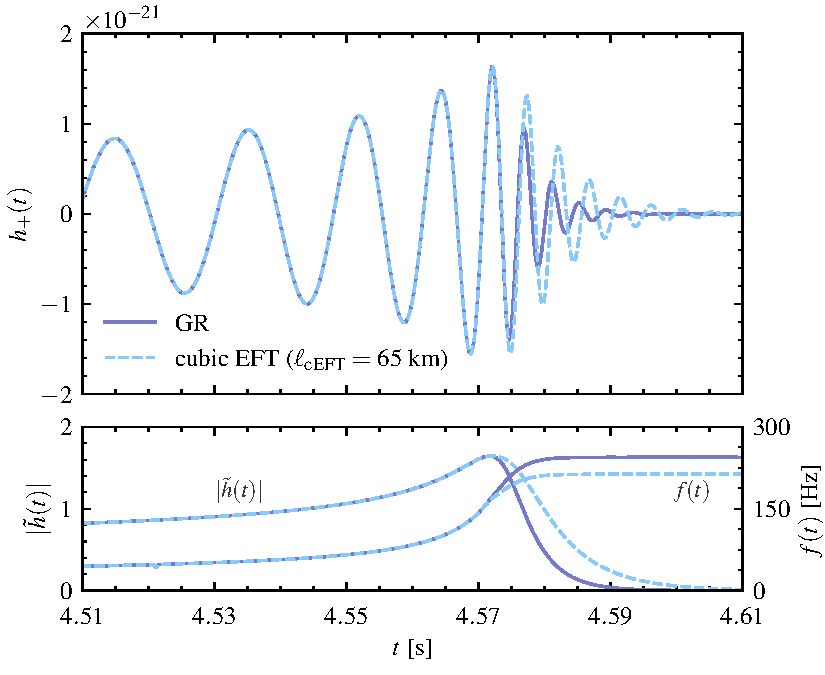
\includegraphics[width=\columnwidth]{figs/example_waveform_cubicEFT.pdf}
\caption{(Color online).~Example GW signal with GW150914-like parameters
for both GR (solid line) and cubic EFT of GR (dashed line) with the leading-order
$n=0$ modifications to the fundamental QNM, for $\ell_{\rm cEFT} = 65$~km.
%
The former is computed with the \SEOB{} model, while the latter with the
\pSEOB{} model, with ringdown modifications according to the results in
Table~\ref{tab:ref_theories_qnms}.
%
Top panel: the $+$ polarization $h_{+}(t)$. Bottom panel: the GW amplitude
$|\tilde{h}(t)|$ (left axes) and the instantaneous frequency $f(t)$ (right axes).
}
\label{fig:example_waveform}
\end{figure}

% \begin{table*}[th]
% \begin{tabular}{c | c c c c c c c c}
% \hline
% \hline
% Theory & $p$ & $\delta \omega^{(0)}_{220}$ & $\delta \tau^{(0)}_{220}$ & $\delta \omega^{(1)}_{220}$ & $\delta \tau^{(1)}_{220}$ & QNM & Constraint & This work \\
% \hline
% EdGB      & 4 & 0.0107 & 0.0044 & $-$0.2480 & $-$1.101 &  \cite{Blazquez-Salcedo:2016enn,Pierini:2021jxd} & $\ell_{\rm GB} \leqslant 1.18$~km~(GW)~\cite{Lyu:2022gdr} & -- \\
% dCS       & 4 & 3.1964 & 6.3619 & 41.199 & 794.66 &  \cite{Wagle:2021tam}   & $\ell_{\rm CS} \leqslant 8.5$~km~(EM+GW)~\cite{Silva:2020acr}  & $\ell_{\rm CS} \leqslant 34.5$~km \\
% cEFT  & 4 & -0.5813  & 2.6469 & -3.8620 & 265.12 & \cite{Cano:2021myl} & \dots  & \dots \\
% qEFT  & 6 & \dots  & \dots & \dots & \dots & \cite{Cano:2021myl} & $\ell_{\rm qEFT} = \dots$~km~\cite{Sennett:2019bpc}  & \dots \\
% \hline
% \hline
% \end{tabular}
% \caption{Summary of the quasinormal modes calculations.
% %
% We summarize each theory we have considered together with: the exponent $p$ at
% which their QNM-modification enters, the corresponding modifications to the
% oscillation frequency $\delta \omega^{(i)}_{220}$ and decay time $\delta \tau^{(i)}_{220}$, the
% references from which we used the results from and the current best constraint
% (if applicable).
% %
% In these cases, the dimensionless parameters $\lambda_{\rm e,o}$ are degenerate
% with the length scale $\ell$.
% %
% }
% \label{tab:ref_theories_qnms}
% \end{table*}

% --------------------------------------------------------------------------------- %
\section{Parameter Inference}
\label{sec:pe}
% In this section, we provide a basic outline of the Bayesian formalism we use to
infer the properties of the underlying GW signal, identify the most promising
events from the catalog of GW observations to base our analyses on, and discuss
the key insights they provide in constraining predictions of modified gravity
theories.

\subsection{Bayesian formalism}
If we assume that a GW signal observed in detector data $d$ is accurately
described by our waveform model \pSEOB{}, we can infer the parameters of the
model, $\bm{\lambda}$, given the hypothesis $\mathcal{H}$, using the Bayes
theorem,
%
\begin{equation}
P(\bm{\lambda} \vert d, \mathcal{H}) =
\frac{p(\bm{\lambda} \vert \mathcal{H}) \, \mathcal{L}(d \vert \bm{\lambda},\mathcal{H})}{E(d \vert \mathcal{H})}\,,
\label{eq:bayes}
\end{equation}
%
where $P(\bm{\lambda} \vert d, \mathcal{H})$ is the posterior probability distribution,
$p(\bm{\lambda} \vert \mathcal{H})$ the prior,
$\mathcal{L}(d \vert \bm{\lambda},\mathcal{H})$ the likelihood, and
$E(d \vert \mathcal{H})$ the evidence.
%
The set of parameters, $\bm{\lambda}$ is a union of the GR waveform
model parameters~$\bm{\theta}$ (c.f.  Sec.~\ref{sec:review_pSEOB}), and
$\ell$,  the only non-GR parameter in this problem which, we recall, set
the characteristic length-scale in which deviations from
GR become relevant in each of the theories described in
Sec.~\ref{sec:review_theories}. Hence,
%
\begin{equation}
\bm{\lambda} = \{\ell\} \cup \{\bm{\theta}\}.
\label{eq:def_params}
\end{equation}

% As discussed in Secs.~\ref{sec:review_theories} and \ref{sec:theory_specific_qnm}, there is a single coupling
% constants in the cases of EdGB and dCS theories, but two in the cubic and
% quartic EFTofGR.
% %
% We also hold the other beyond-GR parameters, $\{\delta \omega_k^{(j)}\},$ and $\{\delta \tau_k^{(j)}\}$
% fixed to theory-specific predictions. Hence, our set of beyond--GR parameters only includes the parameter $\{\ell \}$.
% %

Assuming stationary Gaussian noise, we can write the (log) likelihood function as,
%
\begin{equation}
\ln \mathcal{L}(d \vert \bm{\lambda},\mathcal{H}) \propto
- \tfrac{1}{2}
\langle
d - h(\bm{\lambda}) \vert d - h(\bm{\lambda})
\rangle\,,
\end{equation}
%
with noise-weighted inner product $\langle \cdot | \cdot \rangle$ defined as,
%
\begin{equation}
\langle A | B \rangle =
\int_{f_{\rm low}}^{f_{\rm high}} \, \dd f \,
\frac{\tilde{A}^{\ast}(f) \tilde{B}(f) + \tilde{A}(f) \tilde{B}^{\ast}(f)}{S_{n}(f)}\,,
\end{equation}
%
where $\tilde{A}(f)$ is the Fourier transform of $A(t)$, the asterisk denotes
complex conjugation and $S_{n}(f)$ is the power spectrum density of the
detector.
%
Assuming a specific prior distribution for our parameters (discussed further in the subsequent section), we stochastically
sample over the parameter space using a Markov-Chain Monte Carlo algorithm as implemented in
\texttt{LALInferenceMCMC}~\cite{Rover:2006ni,vanderSluys:2008qx},
a package part of the \texttt{LALInference} software suite~\cite{Veitch:2014wba,lalsuite}.
%
We subsequently marginalize over the remaining parameters to obtain the
posterior probability distribution function~(PDF) on $\ell$,  $P_j(\ell \vert d_j,\mathcal{H})$, our main parameter of interest.
%
% An example of this is shown in Fig. XX.

For $N$ independent GW observations $\{d_j\}$, $j=1,...,N$, each characterised by a posterior probability distribution $P_j(\ell \vert d_j,\mathcal{H})$, the joint posterior can be written as:
%
\begin{equation}
P(\ell | \{d_j\}) = p(\ell) \prod_{j=1}^{N} \frac{P_j(\ell | d_j)}{p_j(\ell)}\,.
\label{eq:cumulative_dist_ell}
\end{equation}
%
where $p_j(\ell)$ are the priors used for each observation, and $p(\ell)$ is an overall prior.
%
Since we assume a uniform prior on $\ell$, the joint posterior is identically
equal to the joint likelihood.
%
In some cases, we found it necessary to work with different prior ranges across
different events, within the context of a given theory.
%
In this situation, when combining the posteriors we use chose as our overall
prior the widest one among the individual events.

\subsection{Priors}

The prior probability distribution functions on the GR parameters are assumed to be uniform over the component masses, $(m_1, m_2)$, isotropically distributed on a sphere in the sky for the source location with $p(d_L) \propto d_L^2$, and isotropic on the binary orientation, $p(\iota, \psi, \phi_0) \propto \sin\iota$. For the spins $(\chi_1, \chi_2)$, we assume a prior uniform and isotropic in the spin magnitudes and restrict ourselves to the $z$-components.
This spin-prior choice can be specified in \texttt{LALInference} using the option \texttt{alignedspin-zprior}.
%
The prior on $t_0$ is uniform and its range is informed by our detection pipelines.

Among our beyond-GR parameters, $\{\ell, \delta \omega_k^{(n)}\delta \tau_k^{(n)}\}$,
as already mentioned in the previous section, we hold $\{\delta \omega_k^{(n)}\}$
and $\{\delta \tau_k^{(n)}\}$ fixed to theory-specific predictions, and allow only $\ell$
to freely vary.
%
For such cases, we assume a prior uniform between appropriate ranges on $\ell$,
making sure that our marginalized posterior distributions on $\ell$ do not rail
over the maximum prior value on $\ell$.


\subsection{Event selection}

\begin{figure}[t]
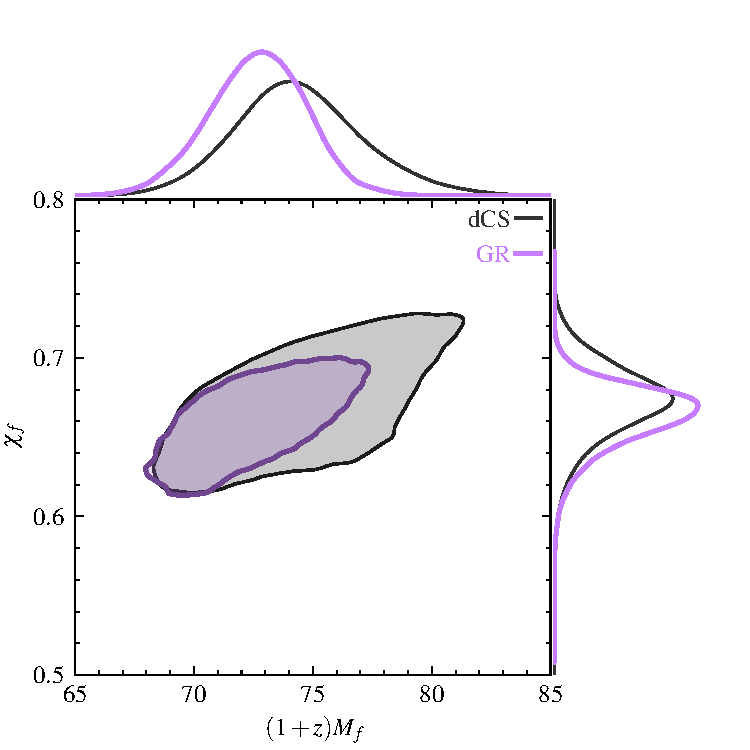
\includegraphics[width=0.9\columnwidth]{figs/tmp_GW150914_intrinsic_params_remnant.pdf}
\caption{(Color online).~Corner plot showing that the inferred final spin $\chi_f$,
detector-frame remnant mass $(1 + z) \, M_f$ for GW150915, using the same waveform model,
but without (blue contours) and with the non-GR parameters different from zero (orange contours, for
dCS gravity and $j=0$). The contours represent 90\% credible regions.
%
We see that the introduction of the non-GR parameters does not bias the
inference on the source parameters.
}
\label{fig:corner_plot}
\end{figure}

The \pSEOB{} model, as described in Sec.~\ref{sec:review_pSEOB}, is an
\emph{IMR} model which infers the properties of the underlying GW signal,
including (independently) its ringdown properties, using the Bayesian formalism
above. Naturally, the most promising candidates for our analyses are high-mass
\emph{and} loud GW observations with a significant signal-to-noise ratio (SNR)
in the post-merger part of the signal.
%
The latest LVK GW catalog~\cite{LIGOScientific:2021djp} reported 90 observed
signals not all of which are relevant for a BH ringdown analysis. In fact, in
an accompanying paper~\cite{LIGOScientific:2021sio}, the \textsc{pSEOBNRv4HM}
analysis\footnote{See, in particular, Sec.VIII A.2
in~\cite{LIGOScientific:2021sio}}, which is most similar to the \pSEOB{} model
presented in this paper, identified two events which provided the strongest
bounds on measurements of the dominant $(220)$ QNM --
GW150914~\cite{LIGOScientific:2016aoc} and
GW200129~\cite{LIGOScientific:2021djp}.
%
These two events, with a total mass of $XX \Mo$ and $XX \Mo$ respectively, are
extremely similar in their source properties. These are also two of the loudest
BBH signals observed to date with a total network SNR of XX and XX
respectively.
%
Moreover, and what is more relevant for our analysis, is their post-inspiral
(merger-ringdown) SNRs, which at XX and XX respectively (see the columns for
$\rho_{\text{post-insp}}$ in Table III of~\cite{LIGOScientific:2019fpa} and
Table IV of~\cite{LIGOScientific:2021sio}).
%
In this paper, we are going to focus on these two GW events as our probes of
the BH ringdown in modified theories of gravity.

The parameter inference in this paper follows configurations identical to the
ones used on these events for the \textsc{pSEOBNRv4HM} analysis in
Ref.~\cite{LIGOScientific:2021sio}. GW150914 was a 2-detector event (HL) while
GW200129 was 3-detector (HLV).
%
We consequently use the same strain data $h(t)$, detector
power-spectral-densities $S_n(f)$ and calibration envelopes as were used for
the analyses in Ref.~\cite{LIGOScientific:2021sio}.
%
The only difference between the sampling configurations is that we do not
sample over the fractional deviations in the $(220)$ QNM frequencies and
damping times, but instead on $\ell$ while holding $\{\delta \omega_k^{(j)}\},$
and $\{\delta \tau_k^{(j)}\}$ fixed to theory-specific predictions.
%
In the section to follow, we enumerate through the different theories and
outline the highlight results. Whenever possible, we also combine results from
multiple events to obtain the strongest possible bound on $\ell$.

% -----------------
% Corner plots here
% -----------------

As a first test ...
\hs{Move to an appendix.}

\subsection{General remarks on the interpretation of our results}
\label{sec:remarks}

There are two conditions that we must take into account before
we can confidently claim to have placed a constraint, within our model's assumptions,
with our parameter estimation study.

First, as we explained in Sec.~\ref{sec:review_theories}, all theories that we
consider must be considered as an effective field theory, meaning it should be
considered valid only below an energy scale, or equivalently, a length scale.
%
As a cut-off length scale for the validity of the EFT we use,
%
\begin{equation}
\Lambda_{\rm EFT} (\varepsilon, \mathfrak{m}) = \varepsilon \, G \mathfrak{m} / c^2 \,,
\label{eq:def_cutoff}
\end{equation}
%
where $\varepsilon$ is a dimensionless number and $\mathfrak{m}$ is the median
value of one of the mass scales involved in the problem.
%
We also momentarily restored factors of $c$ and $G$ to emphasize that $\Lambda_{\rm EFT}$ has
dimensions of length and hence can be compared to the coupling strength $\ell$.
%
In Refs.~\cite{Nair:2019iur,Perkins:2021mhb,Lyu:2022gdr}, $\varepsilon = 1/2$ was used,
but here we consider $\varepsilon \in [0, 1]$.
%
We will say that a bound has been placed on $\ell$, if most of the support of
the posterior distribution function $P(\ell)$ is in the interval
$[0, \, \Lambda_{\rm EFT}(\varepsilon, \mathfrak{m})]$.
%
In practice, this can be quantified through the cumulative distribution function
(CDF) associated with the marginalized posterior distribution $P(\ell)$,
%
\begin{equation}
P(\ell \leqslant \ell_{\rm max}) = \int_{-\infty}^{\,\ell_{\rm max}} P(\ell') \, \dd \ell'\,.
\label{eq:def_cdf}
\end{equation}
%
For instance, we will demand that for a bound with 90\% credibility to be meaningfully placed that
up to $\ell_{\rm max} = \Lambda_{\rm EFT}$ we have,
%
\begin{equation}
% \textrm{CDF}(\ell) \leqslant \textrm{CDF}(T_{\rm EFT}(\varepsilon; \, \mathfrak{m})).
P(\ell \leqslant \Lambda_{\rm EFT}) \leqslant 0.9 \,,
\quad \textrm{(EFT bound)},
\label{eq:eft_bound}
\end{equation}
%
and likewise for other credibility percentiles.

Second, as already emphasized in Ref.~\cite{Maselli:2019mjd}, the ParSpec
formalism is by construction perturbative. This means that the non-GR
deformation parameters are small, that is,
%
\begin{equation}
\gamma \, \delta \omega^{(n)} \ll 1 \,,
\,\, \textrm{and} \,\,
\gamma \, \delta \tau^{(n)} \ll 1 \,, \quad \textrm{(ParSpec bound)},
\label{eq:parspec_bound}
\end{equation}
%
for all orders $n$ in the expansion in dimensionless spin $\chi$ and where $\gamma$
is given by Eq.~\eqref{eq:def_gamma}.
%
We will also construct posterior distributions for these parameters and check if
most of their support is concentrated to a domain with values much smaller than
unity.

Another question we must consider is the following: what is the mass $\mathfrak{m}$ that we should use
in Eq.~\eqref{eq:def_cutoff}?
%
In Refs.~\cite{Nair:2019iur,Perkins:2021mhb,Lyu:2022gdr}, which attempted to
constrain dCS and shift-symmetric sGB theories with the \emph{inspiral} part of
the GW signal alone, it was natural to chose the secondary's mass $m_2$ as the most
conservative choice, since it is (by definition) the smallest mass and hence
places the lowest cut-off scale $\Lambda_{\rm EFT}$ for the validity of either of these theories as an EFT.

In our problem, the answer is not as clear. On the one hand, since we are
interested in the ringdown part of the signal, it is natural to use the
final mass $M_f$ to compute $\Lambda_{\rm EFT}$.
%
On the other hand, one may argue that the modified gravity theory under study
should be able to predict a full inspiral, merger, and ringdown of the black
hole binary before we can even make such a test, and thus the same, more conservative choice
$\gm = m_2$ should be used.
%
Here we adopt an agnostic view to this question and consider \emph{both} masses, $m_2$ and $M_f$, to
determine $\Lambda_{\rm EFT}$. We will then compare how different assumptions
yield to different interpretations of the results of our parameter estimations.


\iffalse
\subsection{Stacking posteriors}
\label{sec:stack}

If, for each event, we find that the constraints~\eqref{eq:eft_bound}
and~\eqref{eq:parspec_bound} are satisfied, we further combine the individual
posteriors distribution on $\ell$, allowing us to place a stronger bound on this parameter.
%
Let us review how do we calculate this \emph{cumulative posterior distribution} on $\ell$.

% 1. Description of data and assumption o \ell being shared
Suppose we have a data set $\{d_{i}\}$ of $N$ events which is described by
model parameters $\bm{\lambda}_{i}$, where $i$ labels each event.
%
We assume that the value of the coupling constant $\ell$, given a specific theory,
is common to all events.
%
% 2. Define joint posterior
%
The joint posterior for the parameters $\bm{\lambda}_{i}$, that describe the
data $\{d_{i}\}$, is
%
\begin{equation}
P(\ell, \{\btheta_i\} | \{d_{i}\})
= \frac{ P(\ell, \{\btheta_i\}) \, P( \{d_i\} | \ell_i, \{\btheta_i\} ) }{ P(\{d_i\}) }.
\label{eq:def_joint_posterior}
\end{equation}
%
where we separated $\ell$ from the GR waveform model parameters $\btheta$ [cf.~Eq.~\eqref{eq:def_params}].
%
% 3. Marginalisation to obtain the cumulative posterior
%
To obtain the cumulative posterior distribution on $\ell$, we marginalize
the joint posterior~\eqref{eq:def_joint_posterior} over
all parameters $\{ \btheta_i \}$, i.e.,
%
\begin{align}
P(\ell | \{d_i\}) &= \int \dd \{\btheta_i\} \, P(\ell, \{\btheta_i\} | \{d_{i}\}),
\nonumber \\
                  &= \int \dd \{\btheta_i\} \, \frac{ P(\ell, \{\btheta_i\}) \, P( \{d_i\} | \ell_i, \{\btheta_i\} ) }{ P(\{d_i\}) },
\nonumber \\
                  &= \frac{P(\ell)}{P(\{d_i\})} \int \dd \{\btheta_i\} \, P(\{\btheta_i\}) \, P( \{d_i\} | \ell, \{\btheta_i\} ),
\end{align}
%
where we have assumed that the prior on $\ell$, $P(\ell)$, is independent of
the other parameters $\{\btheta_i\}$.
%
This allow us to write $P(\ell, \{\btheta_i\} = P(\ell) P(\{\btheta_i\})$
and then move $P(\ell)$ out of the integral
%
We also moved out integral the evidence $P(\{d_i\})$, which is a normalization constant.
%
% 4. Factor the integrals in a product due to statistical independence
%
We can now factor the probabilities inside the integral, since each event is independent from another:
%
\begin{equation}
P(\ell | \{d_i\}) = \frac{P(\ell)}{P(\{d_i\})}
\prod_{i=1}^{N}
\int \dd \btheta_i \, P(\btheta_i) \, P( d_i | \ell_i, \btheta_i ).
\end{equation}
%
% 5. Final formula
We can now identify the integral as the marginalized likelihood for each individual event
%
\begin{equation}
P(\ell | \{d_i\}) = \frac{P(\ell)}{P(\{d_i\})}
\prod_{i=1}^{N} P( d_i | \ell_i ),
\end{equation}
%
which we can rewrite as
%
\begin{align}
P(\ell | \{d_i\}) &= \frac{P(\ell)}{P(\{d_i\})}
\prod_{i=1}^{N} \frac{P(d_i)}{P(\ell_i)} P(\ell_i | d_i)
\nonumber \\
&= P(\ell)
\prod_{i=1}^{N} \frac{P(\ell_i | d_i)}{P(\ell_i)}.
\label{eq:cumulative_dist_ell}
\end{align}
%
by using Bayes' theorem in the first line and cancelling the evidences in the
second line. This is our final result.

%
\hs{Abhirup, maybe move this to the subsection on priors?}
In our parameter estimation runs that we had to adjust our prior on $\ell$ depending on which event and
on which theory we examined.
%
The reasons are twofold.
%
% Describe problem 1
%
First, we found that depending on the source parameters $\btheta$,
large values of $\ell$ could result in unphysical waveforms in the frequency
band we considered. More specifically, these waveforms have a ringdown which is
considerable longer than the inspiral-merger part in the detector frequency band.
%
The fact that our sampled over these waveforms is perhaps not surprising,
because, after all, we are by construction adding corrections to the GR QNM
which \emph{increase} the damping timescale.
%
In practice, we found that these edge-cases were problematic to deal with
\texttt{LALInferenceMCMC}.
%
We overcome this problem, we reduced the prior upper-value of our prior on $\ell$.
%
This choice does not pose a problem to our parameter estimations, because these
waveforms differ grossly from the data and thus have negligible likelihood.
%
% Describe problem 2
%
However, we cannot reduce the prior on $\ell$ too much. If we do so,
to the marginalized posterior distribution on $\ell$ would rail against
the prior or, in a more extreme case, even be a uninformative, flat posterior.
%
% Summary
%
Altogether, this means that the priors $P(\ell)$ are not shared between events and
they must be taken into account when calculation the cumulative posterior function~\eqref{eq:cumulative_dist_ell}.

Finally, we use one of the approaches of Ref.~\cite{Perkins:2021mhb} to
compute the product in Eq.~\eqref{eq:cumulative_dist_ell}.
%
It method relies on first obtaining a kernel density estimator (KDE) for
the posterior distribution on $\ell$ for each individual event.
%
(See also Refs.~\cite{DelPozzo:2011pg,Cardenas-Avendano:2019zxd,Carullo:2021dui}.)
%
Next, we multiply these posteriors according to Eq.~\eqref{eq:cumulative_dist_ell}.
%
This approach based on the KDE can have difficulties in dealing with hard cut-offs in the
distribution, such as the one we impose at $\ell = 0$. We address this issue as
done in Ref.~\cite{Perkins:2021mhb}, by first doubling our number of samples as
$\{ s_i \} \cup \{ - s_i \}$, i.e., mirroring the samples across $\ell = 0$.
%
We then renormalize the associated KDE numerically in the range $\ell = [0, \infty]$.
\fi

% --------------------------------------------------------------------------------- %

In this section, we provide a basic outline of the Bayesian formalism we use to
infer the properties of the underlying GW signal, identify the most promising
events from the catalog of GW observations to base our analyses on, and discuss
the key insights they provide in constraining predictions of modified gravity
theories.

\subsection{Bayesian formalism}
If we assume that a GW signal observed in detector data $d$ is accurately
described by our waveform model \pSEOB{}, we can infer the parameters of the
model, $\bm{\lambda}$, given the hypothesis $\mathcal{H}$, using Bayes' theorem,
%
\begin{equation}
P(\bm{\lambda} \vert d, \mathcal{H}) =
\frac{p(\bm{\lambda} \vert \mathcal{H}) \, \mathcal{L}(d \vert \bm{\lambda},\mathcal{H})}{E(d \vert \mathcal{H})}\,,
\label{eq:bayes}
\end{equation}
%
where $P(\bm{\lambda} \vert d, \mathcal{H})$ is the posterior probability distribution,
$p(\bm{\lambda} \vert \mathcal{H})$ the prior,
$\mathcal{L}(d \vert \bm{\lambda},\mathcal{H})$ the likelihood, and
$E(d \vert \mathcal{H})$ the evidence.
%
The set of parameters, $\bm{\lambda}$ is a union of the GR waveform
model parameters~$\bm{\theta}$ (c.f.  Sec.~\ref{sec:review_pSEOB}), and
$\ell$,  the only non-GR parameter in this problem which, we recall, sets
the characteristic length-scale in which deviations from
GR become relevant in each of the theories described in
Sec.~\ref{sec:review_theories}. %Hence,
%
%\begin{equation}
%\bm{\lambda} = \{\ell\} \cup \{\bm{\theta}\}.
%\label{eq:def_params}
%\end{equation}

% As discussed in Secs.~\ref{sec:review_theories} and \ref{sec:theory_specific_qnm}, there is a single coupling
% constants in the cases of EdGB and dCS theories, but two in the cubic and
% quartic EFTofGR.
% %
% We also hold the other beyond-GR parameters, $\{\delta \omega_k^{(j)}\},$ and $\{\delta \tau_k^{(j)}\}$
% fixed to theory-specific predictions. Hence, our set of beyond--GR parameters only includes the parameter $\{\ell \}$.
% %

Assuming stationary Gaussian noise, we can write the (log) likelihood function as,
%
\begin{equation}
\ln \mathcal{L}(d \vert \bm{\lambda},\mathcal{H}) \propto
- \tfrac{1}{2}
\langle
d - h(\bm{\lambda}) \vert d - h(\bm{\lambda})
\rangle\,,
\end{equation}
%
with the noise-weighted inner product $\langle \cdot | \cdot \rangle$ defined as,
%
\begin{equation}
\langle A | B \rangle =
\int_{f_{\rm low}}^{f_{\rm high}} \, \dd f \,
\frac{\tilde{A}^{\ast}(f) \tilde{B}(f) + \tilde{A}(f) \tilde{B}^{\ast}(f)}{S_{n}(f)}\,,
\end{equation}
%
where $\tilde{A}(f)$ is the Fourier transform of $A(t)$, the asterisk denotes
complex conjugation, $S_{n}(f)$ is the power spectrum density of the
detector \ag{and $[f_{\rm low}, f_{\rm high}]$ span the detector sensitivity band.}
%
Assuming a specific prior distribution for our parameters (discussed further in the next section), we stochastically
sample over the parameter space using a Markov-Chain Monte Carlo algorithm as implemented in
\texttt{LALInferenceMCMC}~\cite{Rover:2006ni,vanderSluys:2008qx} as part of the \texttt{LALInference} software suite~\cite{Veitch:2014wba,lalsuite}.
%
We subsequently marginalize over the remaining parameters to obtain the
posterior probability distribution function~(PDF) on $\ell$,  i.e., $P(\ell \vert d,\mathcal{H})$,
our main parameter of interest.

For $N$ independent GW observations $\{d_j\}$, $j=1,...,N$, each characterised
by a PDF $P_j(\ell \vert d_j,\mathcal{H})$, the
joint posterior can be written as:
%
\begin{equation}
P(\ell | \{d_j\},\mathcal{H}) = p(\ell) \prod_{j=1}^{N} \frac{P_j(\ell | d_j,\mathcal{H})}{p_j(\ell|\mathcal{H})}\,.
\label{eq:cumulative_dist_ell}
\end{equation}
%
where $p_j(\ell | \mathcal{H})$ are the priors used for each observation, and $p(\ell | \mathcal{H})$ is an overall prior.
%
Since we assume a uniform prior on $\ell$, the joint posterior is 
equal to the joint likelihood. Hereafter, we will drop the explicit usage of
$\mathcal{H}$.
%
%In some cases, we found it necessary to work with different prior ranges across
%different events, within the context of a given theory.
%
%In this situation, when combining the posteriors we use chose as our overall
%prior the widest one among the individual events.


\subsection{Priors}

The prior distribution functions on the GR parameters are assumed to be 
uniform over the component masses, $(m_1, m_2)$, isotropically distributed on a 
sphere in the sky for the source location with $p(d_L) \propto d_L^2$, and isotropic 
on the binary orientation, $p(\iota, \psi, \phi_0) \propto \sin\iota$. For the spins 
$(\chi_1, \chi_2)$, we assume a prior uniform and isotropic in the spin magnitudes and restrict ourselves to the $z$-components.
\footnote{\ag{This spin-prior choice can be specified in \texttt{LALInference} using the option \texttt{alignedspin-zprior}.}}
%
%The prior on $t_0$ is uniform and its range is informed by our detection pipelines.

Among our beyond-GR parameters $\{\ell, \delta \omega^{(n)}\delta \tau^{(n)}\}$,
as already mentioned in the previous section, we hold $\{\delta \omega^{(n)},\delta \tau^{(n)}\}$ 
fixed to theory-specific predictions, and only allow $\ell$ to vary freely.
%
We assume an uniform prior on $\ell$ between appropriate ranges,
say $\ell \in [0, \ell_{\rm max}]$.
%
The lower limit is set by the fact the modified gravity theories we consider
all have $p$ even and hence we can assume $\ell > 0$ without loss of
generality.
%
%The upper limit is chosen as to make sure that our marginalized posterior
%distributions on $\ell$ do not rail against $\ell_{\rm max}$.


\subsection{Event selection}

\begin{figure}[t]
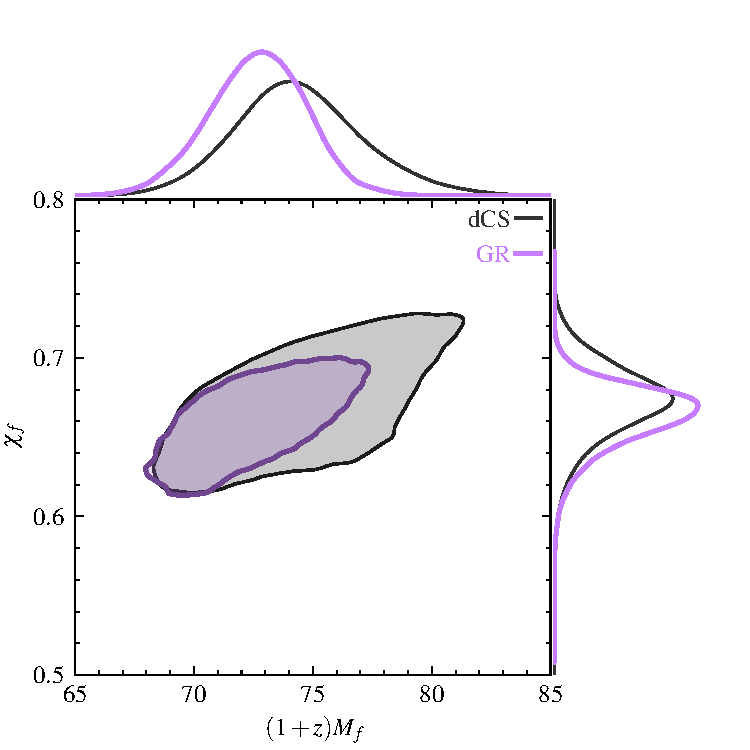
\includegraphics[width=0.9\columnwidth]{figs/tmp_GW150914_intrinsic_params_remnant.pdf}
\caption{(Color online).~Corner plot showing that the inferred final spin $\chi_f$,
detector-frame remnant mass $(1 + z) \, M_f$ for GW150915, using the same waveform model,
but without (blue contours) and with the non-GR parameters different from zero (orange contours, for
dCS gravity and $j=0$). The contours represent 90\% credible regions.
%
We see that the introduction of the non-GR parameters does not bias the
inference on the source parameters.
}
\label{fig:corner_plot}
\end{figure}

The \pSEOB{} model, as described in Sec.~\ref{sec:review_pSEOB}, is an
\emph{IMR} model which infers the properties of the underlying GW signal,
including (independently) its ringdown properties, using the Bayesian formalism
above. Naturally, the most promising candidates for our analyses are high-mass
\emph{and} loud GW observations with a significant signal-to-noise ratio (SNR)
in the post-merger part of the signal.
%
The latest LVK GW catalog~\cite{LIGOScientific:2021djp} reported 90 observed
signals not all of which are relevant for a BH ringdown analysis. In fact, in
an accompanying paper~\cite{LIGOScientific:2021sio}, the \textsc{pSEOBNRv4HM}
analysis\footnote{See, in particular, Sec.VIII A.2
in~\cite{LIGOScientific:2021sio}}, which is most similar to the \pSEOB{} model
presented in this paper, identified two events which provided the strongest
bounds on measurements of the dominant $(220)$ QNM:
GW150914~\cite{LIGOScientific:2016aoc} and
GW200129~\cite{LIGOScientific:2021djp}.
%
These two events, with a total (source-frame) mass of $65 \Mo$ and $63.4 \Mo$ respectively, are
extremely similar in their source properties. These are also two of the loudest
BBH signals observed to date with a total network SNR of 24 and 26.8
respectively.
%
Moreover, and what is more relevant for our analysis, are their post-inspiral
(merger-ringdown) SNRs which are both $\sim `6$ (see the columns for
$\rho_{\text{post-insp}}$ in Table III of~\cite{LIGOScientific:2019fpa} and
Table IV of~\cite{LIGOScientific:2021sio}).
%
In this paper, we are going to focus on these two GW events as our probes of
the BH ringdown in modified theories of gravity.

The parameter inference in this paper follows configurations identical to the
ones used on these events for the \textsc{pSEOBNRv4HM} analysis in
Ref.~\cite{LIGOScientific:2021sio}. GW150914 was a 2-detector  (HL) event while
GW200129 was 3-detector (HLV).
%
We consequently use the same strain data $h(t)$, detector
power-spectral-densities $S_n(f)$ and calibration envelopes as were used for
the analyses in Ref.~\cite{LIGOScientific:2021sio}.
%
%The only difference between the sampling configurations is that we do not
%sample over the fractional deviations in the $(220)$ QNM frequencies and
%damping times, but instead on $\ell$ while holding $\{\delta \omega_k^{(j)}\},$
%and $\{\delta \tau_k^{(j)}\}$ fixed to theory-specific predictions, summarized
%in Table~\ref{tab:ref_theories_qnms}.
%
\sout{In Fig.~\ref{fig:corner_plot}, we show the final spin $\chi_f$ and
detector-frame remnant mass $(1 + z) M_f$ for GW150914 for GR and the
illustrative case of dCS gravity. We see that our waveform models does not
introduce a substantial change to the GR estimates on this parameters, as
required by the ParSpec expansion (see discussion in
Sec.~\ref{sec:review_parspec}).}\agcomm{This reference to Fig.2 appears misplaced here. IMO, Fig 2. has two purposes. 1) to show that we do not need the high-spin version of the fits Carullo used, because our spin posteriors are well-localised around 0.7, and 2) to assure the reader that we were right in using the GR values of the final mass and spin in the ParSpec expansion, because introducing nonGR parameters has not ended up biasing our estimates of Mf-chif.  I think both of these points can be addressed in the discussions section. That is also where we can put the other corner plot with the remaining intrinsic parameters. One side-advantage of this is that the figures would then also appear slightly later in the paper, as we had originally planned.}
%
In Sec.~\ref{sec:results}, we will enumerate through the different theories and
outline the highlight results. Whenever possible, we also combine results from
multiple events to obtain the strongest possible bound on $\ell$.

% -----------------
% Corner plots here
% -----------------

% As a first test ...
% \hs{Move to an appendix.}

\subsection{General remarks on the interpretation of our results}
\label{sec:remarks}

There are two conditions that we must verify before we can confidently claim to
have placed a constraint on $\ell$. First, as we explained in Sec.~\ref{sec:review_theories}, all theories that we
consider must be considered as an effective field theory, meaning it should be
considered valid only below an energy scale, or equivalently, a length-scale.
%
As a cut-off length-scale for the validity of the EFT we use,
%
\begin{equation}
\Lambda_{\rm EFT} (\varepsilon, \mathfrak{m}) = \varepsilon \, G \mathfrak{m} / c^2 \,,
\label{eq:def_cutoff}
\end{equation}
%
where $\varepsilon$ is a dimensionless number and $\mathfrak{m}$ is the median
value of one of the mass scales involved in the problem.
%
We also momentarily restored factors of $c$ and $G$ to emphasize that $\Lambda_{\rm EFT}$ has
dimensions of length and hence can be compared to the coupling strength $\ell$ \agcomm{Note, that we have also restored G,c factors in Eq.3.3}.
%
In Refs.~\cite{Nair:2019iur,Perkins:2021mhb,Lyu:2022gdr}, $\varepsilon = 1/2$ was used,
but here we consider $\varepsilon \in [0, 1]$ for generality.
%
We will say that a bound has been placed on $\ell$, if most of the PDF $P(\ell | d)$ support is in the interval
$[0, \, \Lambda_{\rm EFT}(\varepsilon, \mathfrak{m})]$.
%
In practice, this can be quantified through the cumulative distribution function
(CDF) associated with the marginalized posterior distribution $P(\ell | d)$, namely
%
\begin{equation}
% P(\ell \leqslant \ell_{\rm max}) = \int_{-\infty}^{\,\ell_{\rm max}} \dd \ell'\, P(\ell') \,.
% HS: changed lower limit to zero since we don't have support for negative \ell-values
P(\ell \leqslant \ell_{\rm max} | d) = \int_{0}^{\,\ell_{\rm max}} \dd \ell'\, P(\ell' | d) \,.
\label{eq:def_cdf}
\end{equation}
%
For instance, we will require that for a bound with 90\% credibility to be placed on $\ell$ that
%
\begin{equation}
% \textrm{CDF}(\ell) \leqslant \textrm{CDF}(T_{\rm EFT}(\varepsilon; \, \mathfrak{m})).
P(\ell \leqslant \Lambda_{\rm EFT} | d) \leqslant 0.9 \,,
\quad \textrm{(EFT bound)},
\label{eq:eft_bound}
\end{equation}
%
where we let $\ell_{\rm max} = \Lambda_{\rm EFT}$ in Eq.~\eqref{eq:def_cdf}, and
likewise for other credibility percentiles\agcomm{Note that we were using $\ell_{\rm max}$
in the previous section to denote the upper end of the prior. I suggest that we remove the 
$\ell_{\rm max}$ reference from the previous section. No need to go into details about prior
boundaries.}.

Second, as already emphasized in Ref.~\cite{Maselli:2019mjd}, the ParSpec
formalism is by construction perturbative. This means that the non-GR
deformation parameters are small, that is,
%
\begin{equation}
\gamma \, \delta \omega^{(n)} \ll 1 \,,
\,\, \textrm{and} \,\,
\gamma \, \delta \tau^{(n)} \ll 1 \,, \quad \textrm{(ParSpec bound)},
\label{eq:parspec_bound}
\end{equation}
%
for all orders $n$ in the expansion in dimensionless spin $\chi$ and where $\gamma$
was defined in Eq.~\eqref{eq:def_gamma}.
%
We will also construct posterior distributions for these parameters and check if
most of their support is concentrated to a domain with values much smaller than
unity.

Another question we must consider is the following: what is the mass $\mathfrak{m}$ that we should use
in Eq.~\eqref{eq:def_cutoff}?
%
In Refs.~\cite{Nair:2019iur,Perkins:2021mhb,Lyu:2022gdr}, which attempted to
constrain dCS and EdGB theories with the \emph{inspiral} part of
the GW signal alone, it was natural to choose the secondary's mass $m_2$ as the most
conservative choice, since it is by definition the smaller component mass and hence
places the lowest cut-off scale $\Lambda_{\rm EFT}$ for the validity of either of these theories as an EFT.

In our problem, the answer is not as clear. On the one hand, since we are
interested in the ringdown part of the signal, it is natural to use the
final mass $M_f$ to compute $\Lambda_{\rm EFT}$.
%
On the other hand, one may argue that the modified gravity theory under
consideration should be able to predict a full inspiral, merger, and ringdown
of the black hole binary before we can even make such a test, and thus the
same, more conservative choice $\gm = m_2$ should be used.
%
Here we adopt a pragmatic approach to this issue and consider \emph{both}
masses, $m_2$ and $M_f$, to determine $\Lambda_{\rm EFT}$.
%
We will then compare how different assumptions yield to different
interpretations of the results of our parameter estimation.



%%%%%%%%%%%%%%%%%%%%%%%%%%%%%%%%%%%%%%%%%
\section{Results using LIGO-Virgo events}
\label{sec:results}
%%%%%%%%%%%%%%%%%%%%%%%%%%%%%%%%%%%%%%%%%

% ----------------------------------------------------------
% \hs{Convention: us 90\% credibility for the final bounds.}
% ----------------------------------------------------------

% -----------------
% Explain threshold
% -----------------


% \hs{Note to ourselves: as mentioned in~\cite{Maselli:2019mjd}:
% %
% ``As customary in parametrized approaches, we focus on perturbative corrections by assuming $\gamma_{i} \delta \omega^{(n)} \ll 1$, $\gamma_{i} \delta \tau^{(n)} \ll 1$ and GR is recovered in the limit $\gamma_{i} \to 0$.''
% We should check this \emph{in addition} to the small-coupling approximation to argue whether we placed a bound or not.
% }

\subsection{Einstein-dilaton-Gauss-Bonnet gravity}
\label{sec:results_edgb}

We start \sout{by showing our results for} \ag{with} EdGB gravity.
%
In Fig.~\ref{fig:edgb_exec_sum} we show the marginalized PDFs of the
coupling constant $\ell_{\rm GB}$, for GW150914 (top panel) and GW200129
(middle panel), with and without the spin corrections to the $(2,2,0)$ QNM.
%
The bottom panel shows the joint posterior from combining both events.
%
We see, for both events events, the $N_{\rm max} = 0$ posteriors are
characterized by a peak away from zero.
%
This does not mean that we are inferring a deviation from GR.
%
Recall that the deviations from GR in the ParSpec framework are controlled
by $\gamma$, which here reads,
%
\begin{equation}
    \gamma_{\rm GB} = \left(\frac{c^2 \ell_{\rm GB}}{ G M_{f}}\right)^4\,.
    \label{eq:def_gamma_gb}
\end{equation}
%
As shown in Fig.~\ref{fig:gamma_gb}, $\gamma_{\rm GB}$ does indeed have a posterior
distribution with largest support at zero, indicating consistency between \sout{data} 
\ag{the underlying signal} \agcomm{whenever possible, I replaced ``data" when we 
meant signal, simply because earlier we defined data to also include noise, and by a
GR prediction we conventionally refer to the signal. }
and GR.
%
We also observe that the inclusion of the spin corrections (i.e., curves with $N_{\rm max} = 1$)
displaces the posteriors distributions towards smaller values of $\ell_{\rm GB}$ \ag{(Fig.~\ref{fig:edgb_exec_sum}).
and larger values of $\gamma_{\rm GB}$ (Fig.~\ref{fig:gamma_gb}).}

\begin{figure}[t]
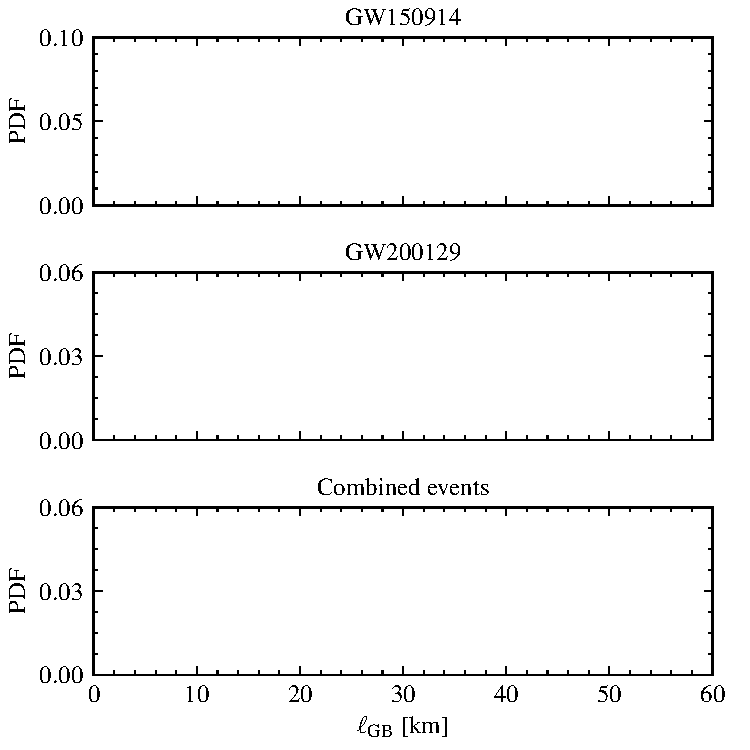
\includegraphics[width=\columnwidth]{figs/edgb_posteriors_combined.pdf}
\caption{(Color online).~Posterior distribution function on coupling constant $\ell_{\rm GB}$ in EdGB gravity
for GW150914 (top panel), GW200129 (middle panel)
and from combining results (bottom panel).
%
In all panels, different line colors correspond to the inclusion ($N_{\rm max} = 1$) or not ($N_{\rm max} = 0$)
of the linear-in-spin QNM correction.
%
The joint posteriors are shown for illustrative purposes only. As we explain in Fig.~\ref{fig:edgb_cdf} and
in the main text, our analysis of these events fails to satisfy the EFT bound~\eqref{eq:eft_bound}.
}
\label{fig:edgb_exec_sum}
\end{figure}

\begin{figure}[h]
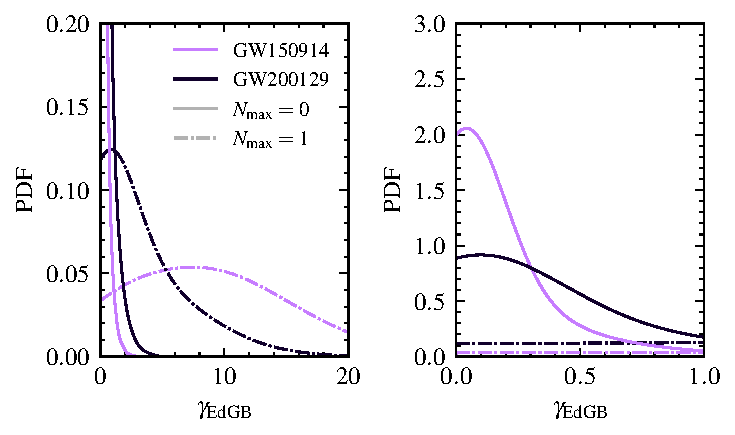
\includegraphics[width=\columnwidth]{figs/edgb_gamma.pdf}
\caption{(Color online).~Posterior distribution function on the dimensionless parameter $\gamma_{\rm GB}$,
defined in Eq.~\eqref{eq:def_gamma_gb}. We see that this parameter controls the ParSpec expansion in EdGB gravity
does have maximum support at $\gamma_{\rm GB} = 0$. This shows that our model is consistent with GR.
\agcomm{I was thinking a bit more about the colors we choose for the plots, and I think Figs. 1-2 should have a different set of colors from Figs. 3-10. That is because the former have GR-nonGR comparisons, while the latter has comparisons between different spin corrections. Casual readers sometimes make an unconscious connection of quantities with colors. }}
\label{fig:gamma_gb}
\end{figure}

\begin{figure}[t]
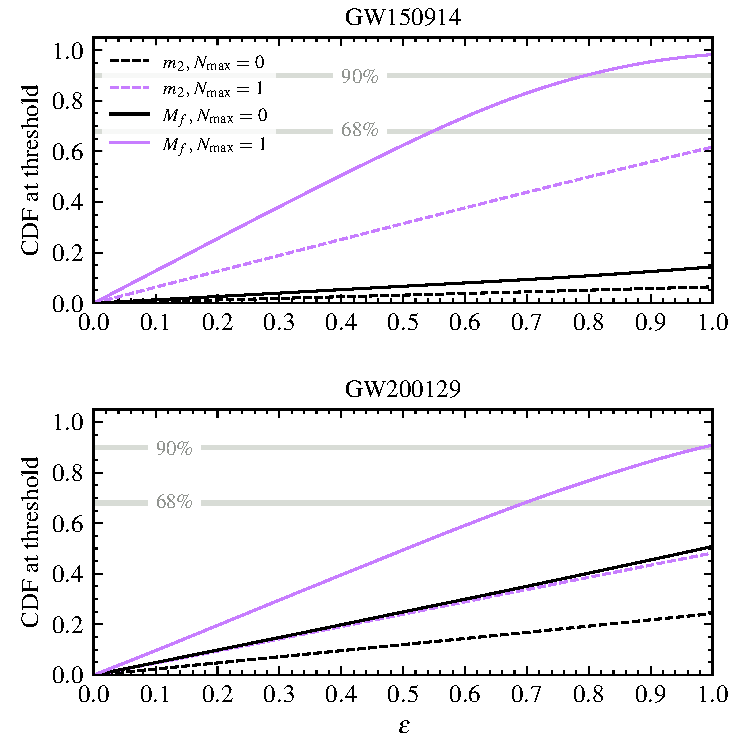
\includegraphics[width=\columnwidth]{figs/edgb_cdf_varying_threshold.pdf}
\caption{(Color online).~The CDF evaluated at the
cut-off $\Lambda_{\rm EFT}(\varepsilon,\gm)$ for EdGB gravity as a function of the parameter
$\varepsilon$ for both (dashed curves) $\gm = m_2$, the secondary's source
mass, and (solid curves) $\gm = M_{f}$, the remnant's source mass, without
(black curves) and with (purple curves) linear in spin QNM corrections. The
horizontal lines \sout{lay at 0.68 and 0.90}\ag{mark the 68\% and 90\% credible levels}. 
We see that in no situation the curves pass
through the 0.68 or 0.90 lines even at $\varepsilon = 1$.
\agcomm{Am I missing something something? The Nmax=1 lines for GW150914 does 
cross the credible levels, as well as the m2 Nmax=1 line for GW200129.}
%
This means that no bound on $\ell_{\rm GB}$ can be placed with the events we
analyzed.
}
\label{fig:edgb_cdf}
\end{figure}

\begin{table}[h]
\begin{tabular}{l l c c c}
\hline
\hline
$N_{\rm max}$ & Event &  EFT    & ParSpec & Constraint      \\
              &       &  bound? & bound?  & ($\gm = M_{f}$) \\
\hline
  & GW150914 & No  & Yes & -- \\
0 & GW200129 & No  & Yes & -- \\
  & Combined & --  & Yes & -- \\
\hline
  & GW150914 & No  & Yes & -- \\
1 & GW200129 & No  & Yes & -- \\
  & Combined & --  & Yes & -- \\
\hline
\hline
\end{tabular}
\caption{Detailed summary of our results for EdGB gravity for GW150914, GW200129, and
combined events using $\gm = M_{f}$, $\varepsilon = 1/2$ and quoting only 90\% credible results.
%
We find that we cannot place any constraint on $\ell_{\rm GB}$ with our waveform model from either GW event.
}
\label{tab:summary_edgb}
\end{table}

As we emphasized in Sec.~\ref{sec:remarks}, we must first check whether the
``EFT''~\eqref{eq:eft_bound} and ``ParSpec''~\eqref{eq:parspec_bound} bounds
are satisfied, before drawing any conclusions on the allowed values for
$\ell_{\rm GB}$ from our parameter estimations.
%
We check the validity of the EFT bound in Fig.~\ref{fig:edgb_cdf}. In the top (bottom) panel we show
the CDF of the $\ell_{\rm GB}$ posteriors for GW150914 (GW200129), obtained
by evaluating the integral~\eqref{eq:def_cdf} with $\ell_{\rm max} = \Lambda_{\rm EFT}(\varepsilon, \mathfrak{m})$,
with the mass scale set by the secondary's mass (i.e., $\mathfrak{m} = m_2$, dashed lines) or
the remnant's mass ($\mathfrak{m} = M_f$, solid lines), while varying $\varepsilon$ between 0 and 1.
%
For GW150914, we see that for the $N_{\rm max} = 0$ curves, that the CDF never goes
past $0.2$, regardless of the mass scale $\mathfrak{m}$ used and even at $\varepsilon =
1$, at which the EFT description of the theory would not be valid anyway.
%
This shows that that the ``EFT bound'' given by Eq.~\eqref{eq:eft_bound} is
never met at a significant credibility and thus that we cannot place a bound on
$\ell_{\rm GB}$.
%
The situation is similar for GW200129 with $N_{\rm max} = 0$ and does not
change for either event when we add spin corrections to the EdGB QNM.
%
Taken together we are led to \emph{conclude that we cannot constrain EdGB gravity with our
present model}.
%
We summarize our findings in Table~\ref{tab:summary_edgb}.

We can compare this conclusion with that of Ref.~\cite{Carullo:2021dui}, which obtained $\ell_{\rm GB} \lesssim 35$~km,
by setting $p=4$, \emph{but not} including theory-specific QNM information on $\delta \omega^{(n)}$ and $\delta \tau^{(n)}$.
%
Our results provide a concrete example of the importance of including
theory-specific QNM calculations information into the parameter estimation
and how this can dramatically change the outcome of the results.

Let us also contrasts our results with those of Refs.~\cite{Nair:2019iur,Perkins:2021mhb,Lyu:2022gdr}
which relied on the BBH inspiral to constrain $\ell_{\rm GB}$, as discussed in Sec.~\ref{sec:review_edgb}.
%
We see that EdGB provides an example of a theory in which the inspiral portion
of the signal is more constraining then the ringdown portion of the signal.
%
Two reasons together can explain our negative results. First, as observed by
Ref.~\cite{Blazquez-Salcedo:2016enn}, the QNMs of EdGB BHs only differ slightly
from their Schwarzschild counterparts. Second, the larger mass $M_f$ of the
remnant BH, suppresses scalar field's charge relatively to the initial binary
components.~\hs{This is a general `limitation' of ringdown test of higher-curvature theories in present detectors.
Point this out in the conclusions after all specific theories are discussed.}
%
As we will next, the situation is the opposite for dCS gravity.

% Let us place our results in a broader context. In particular, let us contrast
% them against those of Ref.~\cite{Lyu:2022gdr} which placed the bound
% %
% $\ell_{\rm GB} \leqslant 1.33$~km
% %
% using the neutron star-black hole binaries GW200105 and GW200115~\cite{LIGOScientific:2021qlt}, and
% of Refs.~\cite{Nair:2019iur,Perkins:2021mhb}, which placed the bound
% %
% $\ell_{\rm GB} \leqslant 1.7$~km,
% %
% by stacking the posterior of $\ell_{\rm GB}$ from a  selection of black hole binaries from the GWTC-1 and GWTC-2 catalogs
% with at least one relatively low-mass binary component~\cite{}\footnote{These bounds
% are, strictly speaking, valid only when the scalar field $\varphi$ is small, i.e., $\varphi \ll 1$, and
% take into consideration only the leading-order scalar field contribution arising from the dilatonic coupling.}.
% %
% These works use the \emph{inspiral} portion of GW event only and a constraint
% on EdGB gravity can be obtained because black holes in this theory carry a
% monopole scalar charge which in turn can source dipolar scalar radiation,
% that affects the GW phase at $-1$PN order, relative to the dominant GR contribution, and
% is proportional to the difference between the charges of binary components.
% %
% Now, the magnitude of the scalar charge scales roughly with the inverse of the black hole's mass squared, that is,
% smaller (larger) back holes carry large (smaller) scalar charges. Qualitatively, this is because the scalar field
% is sourced by the Gauss-Bonnet curvature invariant, which is large for black holes with small masses.
% %
% Beyond-GR corrections to the inspiral are, by construction, not present in our
% waveform model and constitutes a important ingredient to be added in forthcoming
% versions of the model.
% %
% In addition to the larger mass (which suppresses the black hole's charge), the
% QNM of EdGB gravity differ very little from GR as observed in~\cite{Blazquez-Salcedo:2016enn}.
% %
% Hence, here we have an example of a theory in which the inspiral portion of the signal
% is more constraining then the ringdown portion of the signal.
%
% As we will next, the situation is the opposite for dCS gravity.


\subsection{Dynamical Chern-Simons}
\label{sec:results_dcs}

\begin{figure}[t]
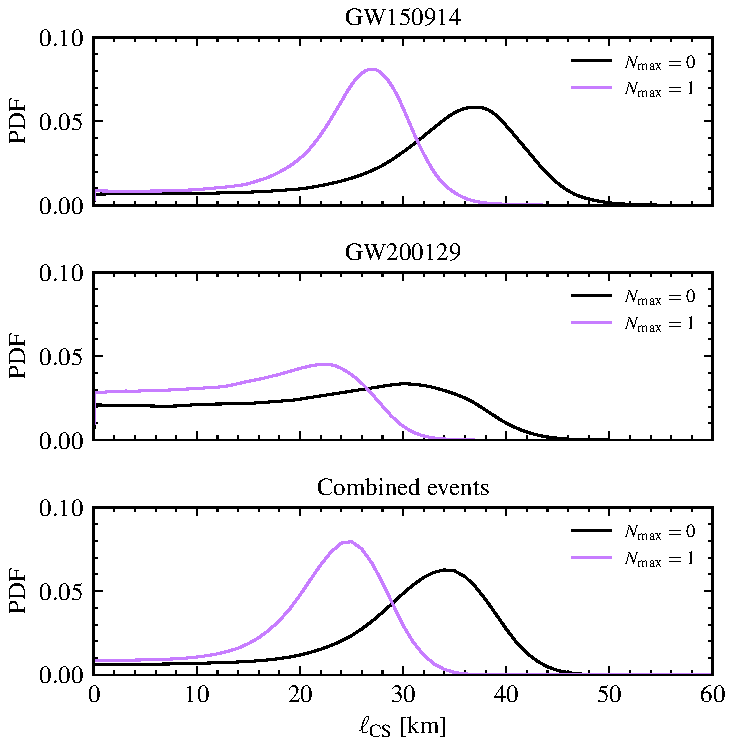
\includegraphics[width=\columnwidth]{figs/dcs_posteriors_combined.pdf}
\caption{(Color online).~Similar to Fig.~\ref{fig:edgb_exec_sum}, but for dCS gravity.
%
% ~Posterior distribution function for the coupling constant $\ell_{\rm CS}$ for
% GW150914 (top panel), GW200129 (middle panel) and combined events (bottom panel).
% %
% In all panels, we use solid and dashed lines to correspond to the inclusion or not of the linear
% in spin QNM correction.
%
We stress that posteriors obtained including $n=1$ corrections, violate conditions~\eqref{eq:parspec_bound}
and therefore should not be used to draw meaningful conclusions. We show them for illustrative purposes
and also to emphasize the importance of taking conditions~\eqref{eq:eft_bound} and~\eqref{eq:parspec_bound}
simultaneously into consideration when analyzing the results of the parameter estimation.
}
\label{fig:dCS_exec_sum}
\end{figure}

\begin{figure}[t]
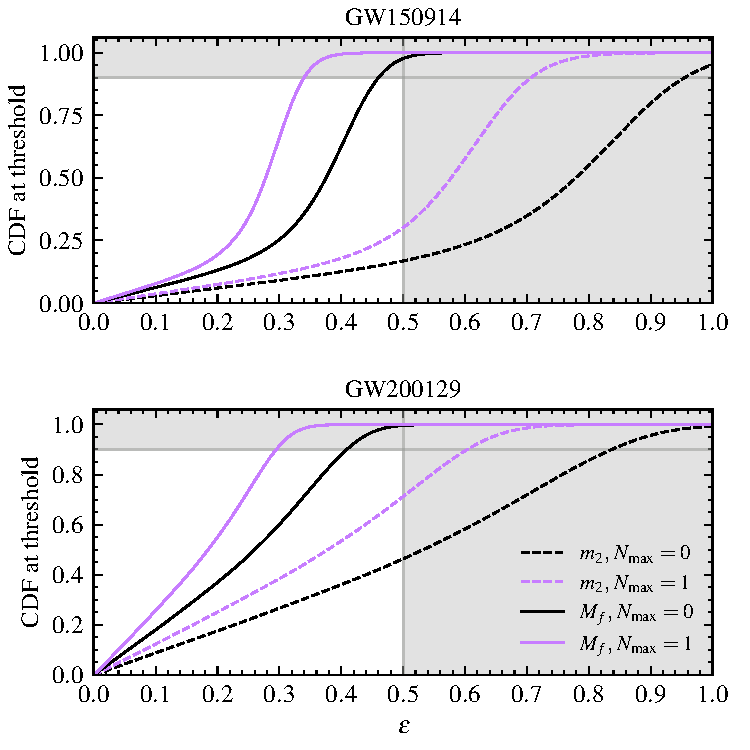
\includegraphics[width=\columnwidth]{figs/dcs_cdf_varying_threshold.pdf}
\caption{(Color online).~Similar to Fig.~\ref{fig:edgb_cdf}, but for dCS gravity.
% The cumulative distribution function evaluated at the
% cut-off $\Lambda_{\rm EFT}(\varepsilon, \gm)$ as a function of the parameter $\varepsilon$ for both
% $\gm = m_2$ (solid and dashed lines) and $\gm = M_{f}$ (dot-dashed and dotted lines) without
% (blue lines) and with (orange lines) linear-in-spin QNM corrections.
% The horizontal lines lay at 0.68 and 0.90.
%
We see that the CDF curves for $\gm = M_{f}$ are above 90\% for $\varepsilon =
1/2$ for both events, with and without including the $n = 1$ dCS corrections to
the dominant QNM.
}
\label{fig:dcs_cdf}
\end{figure}

We now consider dCS gravity \ag{where the main results are summarised in Fig.~\ref{fig:dCS_exec_sum}}.
%
\sout{In Fig.~\ref{fig:dCS_exec_sum} we show the marginalized posterior distribution
function of $\ell_{\rm CS}$ for both events GW150914 (top panel) and GW200129
(middle panel), with different colors distinguishing cases with and without spin corrections to
dominant $(2,2,0)$~QNM.}\agcomm{A lot of the language here is a repetition of the previous section.}
%
\sout{Perhaps the most salient feature of these posteriors is that they are not
peaked at $\ell_{\rm CS}$, which may mislead us to believe that we are seeing a
deviation from GR. This is not the case and the situation is that same as the
one we discussed in the previous section for EdGB gravity.}
\ag{As with EdGB gravity (Sec.~\ref{sec:results_edgb}) although the PDF of $\ell_{\rm CS}$
is peaked away from 0, this does not signify a deviation from GR, as we have verified that,}
%
\sout{We verified that}
%
\begin{equation}
    \gamma_{\rm CS} = \left( \frac{c^2 \ell_{\rm CS}}{G M_{f}} \right)^{4}\,,
\end{equation}
%
does indeed peak at zero indicating consistency with GR, similarly to what is shown in Fig.~\ref{fig:gamma_gb} for $\gamma_{\rm GB}$.
%
We also see that in both cases that the inclusion leading-order-in-spin
correction to the mode displaces the posteriors towards smaller values of
$\ell_{\rm CS}$. This can be seen more evidently by looking at the location of
posterior peaks.
%
Finally, in the bottom panel, we show the combined result for both events.
\agcomm{Just a thought.  Since, Figs 3,6,8,10 and Figs.4,6,9,11 show the same basic thing,
should we have one description at the top of the section for each figure? We can follow this up
by what is special for each theory in each section? Currently, we are repeating a lot of the 
language to describe these figures for each theory?}

In Fig.~\ref{fig:dcs_cdf} we show the CDF
\sout{obtained from Eq.~\eqref{eq:def_cdf}, with $\ell_{\rm max} = \Lambda_{\rm EFT} (\varepsilon, \gm)$,
for both GW150914 (top panel) and GW200129 (bottom panel), where $\Lambda_{\rm EFT}$
is calculated with either $\gm = m_2$ (dashed lines) or $M_{f}$ (solid lines),
and in the range $\varepsilon \in [0,1]$.}
%
\sout{For}\ag{for} GW150914, we see that with $\gm = m_2$ that Eq.~\eqref{eq:eft_bound} is not
satisfied unless $\varepsilon \approx 0.9$ (with only $n=0$ corrections) and
$\varepsilon \approx 0.7$ (with both $n=0$ and $1$ corrections).
%
The situation is different if we use $\gm = M_f$. In this case, we find that
with or without spin corrections that Eq.~\eqref{eq:eft_bound} can be satisfied
with $\varepsilon \leqslant 1/2$, i.e., below the criteria used
Refs.~\cite{Nair:2019iur,Perkins:2021mhb,Lyu:2022gdr}.
%
This means that with our model's assumptions and using the remnant's source mass $M_f$ to set the
cut-off scale that we can claim an upper bound
%
\begin{equation}
\ell_{\rm CS} \leqslant 42.6~\textrm{km}
\quad \textrm{(90\% credibility)},
\end{equation}
\agcomm{I am not familiar with the term ``credibility", and am more used to the phrase, ``at X\% credible level". 
Are they the same thing?}
%
on dCS gravity and would constitute \emph{the first bound on this theory with
gravitational-wave observations alone}.\agcomm{Since this is an extremely important
result, would it make sense to reorder the theories such that dCS comes first among results?}
%
We also note that since the CDF grows fast in approximate domain $\varepsilon = [0.2, 0.4]$,
that a stronger, albeit at lower credibility,
%
\begin{equation}
\ell_{\rm CS} \leqslant 37.4~\textrm{km}
% ~( = \Lambda_{\rm EFT}(0.3, M_{f}) )
\quad \textrm{at 68\% credibility},
\end{equation}
%
can also be placed, when $N_{\rm max}=0$.

We can draw qualitatively similar conclusions from the GW200129 event.
In particular, we find,
%
\begin{equation}
\ell_{\rm CS} \leqslant 36.6~\textrm{km}
% 43.9~\textrm{km}~( = \Lambda_{\rm EFT}(\tfrac{1}{2}, M_{f}) )
\quad \textrm{(90\% credibility)},
\end{equation}
%
and
%
\begin{equation}
\ell_{\rm CS} \leqslant 29.1~\textrm{km}
% ~( = \Lambda_{\rm EFT}(0.3, M_{f}) )
\quad \textrm{(68\% credibility)},
\end{equation}
%
when $N_{\rm max}=0$.
%
These stronger bounds are a consequence of the larger support for $\ell_{\rm CS} \lessapprox 15$~km
for GW200129 (compare the top and middle panels in Fig.~\ref{fig:dCS_exec_sum}), and in part due to
the smaller median remnant ($M_{f} \approx 59.5\msun$ versus $M_{f} \approx 61.8\msun$ for GW150914).
%
\hs{Should we remove these and just quote the 90\% results?}\agcomm{I think
it's fine to give point estimates, because it's easier for reader to interpret results 
rather than having to make sense of error bars.}

We also found for both GW events, that the
perturbative-conditions~\eqref{eq:parspec_bound} required by the ParSpec
formalism is violated for the $\gamma_{\rm CS} \, \delta \tau^{(1)}$ coefficient.
%
This means that we cannot use these posterior to infer any meaningful bound on dCS gravity
and that is why we quoted only the $N_{\rm max}=0$ bound above.

Finally, since both events individually led to a bound on $\ell_{\rm CS}$
(assuming a cut-off scale for $\gm = M_{f}$ and $N_{\rm max}=0$), we can combine the
posteriors to obtain the cumulative bound,
%
\begin{equation}
\ell_{\rm CS} \leqslant 38.7~\textrm{km}
\quad \textrm{(90\% credibility)},
\end{equation}
%
which is the main result of this section.
%
This bound is approximately a factor of four weaker than that placed by
Ref.~\cite{Silva:2020acr}, but
%
(i) relies only on GW observations and
%
(ii) suggests that a ringdown analysis can potentially place constraints on
theories which evade GW tests using inspiral information alone, such as the
case of dCS gravity~\cite{Nair:2019iur,Perkins:2021mhb,Lyu:2022gdr}.
%
In Table~\ref{tab:summary_dcs} we summarize our findings of this section.

\begin{table}[h]
\begin{tabular}{l l c c c}
\hline
\hline
$N_{\rm max}$ & Event & EFT    & ParSpec & Constraint ($\gm = M_{f}$) \\
              &       & bound? & bound?  &                            \\
\hline
%       & GW150914 & Yes & Yes & $\ell_{\rm CS} \leqslant 46.5$~km \\
% 0     & GW200129 & Yes & Yes & $\ell_{\rm CS} \leqslant 43.9$~km \\
%       & Combined & Yes & Yes & \cellcolor{blue!10}$\ell_{\rm CS} \leqslant 34.5$~km \\
      & GW150914 & Yes & Yes & $\ell_{\rm CS} \leqslant 41.9$~km \\
0     & GW200129 & Yes & Yes & $\ell_{\rm CS} \leqslant 35.8$~km \\
      & Combined &     &     & \cellcolor{black!10}$\ell_{\rm CS} \leqslant 38.7$~km \\
\hline
      & GW150914 & Yes & No  & --                                 \\
1     & GW200129 & Yes & No  & --                                 \\
      & Combined &     &     & --                                 \\
\hline
\hline
\end{tabular}
\caption{Detailed summary of our results for dCS gravity for GW150914, GW200129, and
combined events using $\gm = M_{f}$, $\varepsilon = 1/2$ and quoting only 90\% credible bounds.
%
We found that while our posteriors satisfy the condition~\eqref{eq:eft_bound} (with $\varepsilon = 1/2$),
they do not obey the condition~\eqref{eq:parspec_bound} for $N_{\rm max} = 1$. This means
that our results for $N_{\rm max}=0$ are the only ones we can confidently quote.
%
The combined bound, which is also quoted in Table~\ref{tab:ref_theories_qnms},
is $\ell_{\rm CS} \leqslant 38.7$~km.
}
\label{tab:summary_dcs}
\end{table}

\subsection{Cubic Effective-Field-Theory of General Relativity}
\label{sec:results_ceft}

We now consider the cubic EFT of GR.
%
In Fig.~\ref{fig:cEFT_exec_sum} we show the marginalized posterior distributions
functions of $\ell_{\rm cEFT}$ for GW150914 (top panel) and GW200129 (middle panel),
with different curve colors corresponding to different $N_{\rm max}$ in
the spin expansion.
%
We find that in this theory, the posterior distributions are mostly uniform for
$\ell_{\rm cEFT} \lesssim 40$~km (contrast this with the EdGB and dCS gravity
cases; cf.~Figs.~\ref{fig:edgb_exec_sum} and~\ref{fig:dCS_exec_sum}).
%
For values $\ell_{\rm cEFT} \gtrsim 40$~km, the posteriors smoothly approach zero.

In Fig.~\ref{fig:cEFT_cdf} we show the CDF for both events, calculated in the
same way as already described for the EdGB and dCS theories.
%
We see that curves are very similar to those of dCS gravity for GW200129 (cf.
bottom panel in Fig.~\ref{fig:cEFT_cdf}).
%
Moreover, we find that the EFT~\eqref{eq:eft_bound} and
ParSpec~\eqref{eq:parspec_bound} bounds are satisfied for both events both when
$\mathfrak{m} = M_f$ and $N_{\rm max} = 1/2$.
%
This allows us to place the combined bound of
%
\begin{equation}
    \ell_{\rm cEFT} \leqslant 38.2~\textrm{km}\,,
\end{equation}
%
at 90\% credibility. As also happened for our study for dCS, the find that for
the cubic EFT that the ParSpec bound is violated by the $n = 1$ corrections to
the QNMs, meaning that we cannot use this case to draw any meaningful
constraint on this parameter.
%
We summarize our results in Table~\ref{tab:summary_ceft}.

\begin{figure}[t]
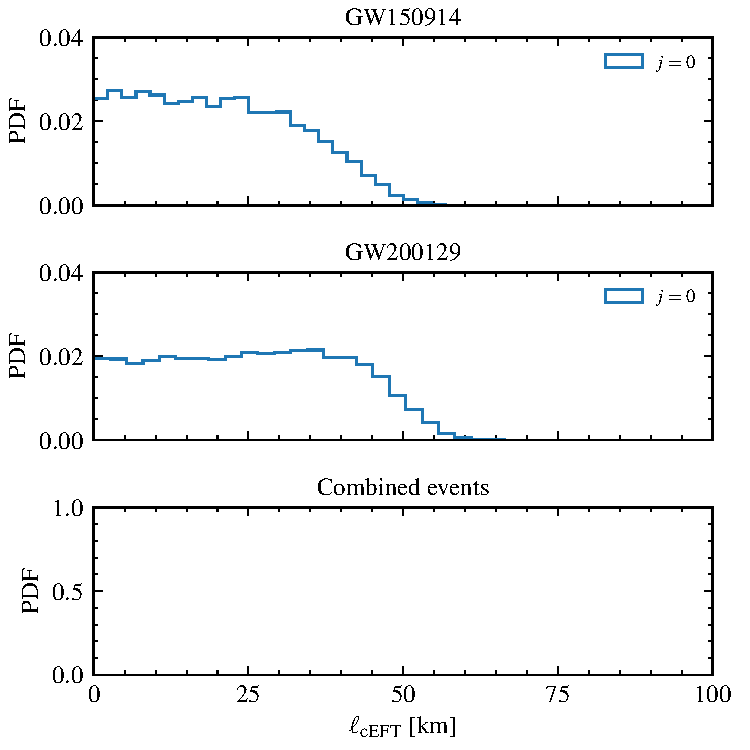
\includegraphics[width=\columnwidth]{figs/ceft_posteriors_combined.pdf}
\caption{(Color online).~Posterior distribution function for the coupling constant $\ell_{\rm cEFT}$ for
GW150914 (top panel), GW200129 (middle panel) and combined events (bottom panel).
%
The colors distinguish different $N_{\rm max}$ in the spin expansion.
}
\label{fig:cEFT_exec_sum}
\end{figure}

\begin{figure}[t]
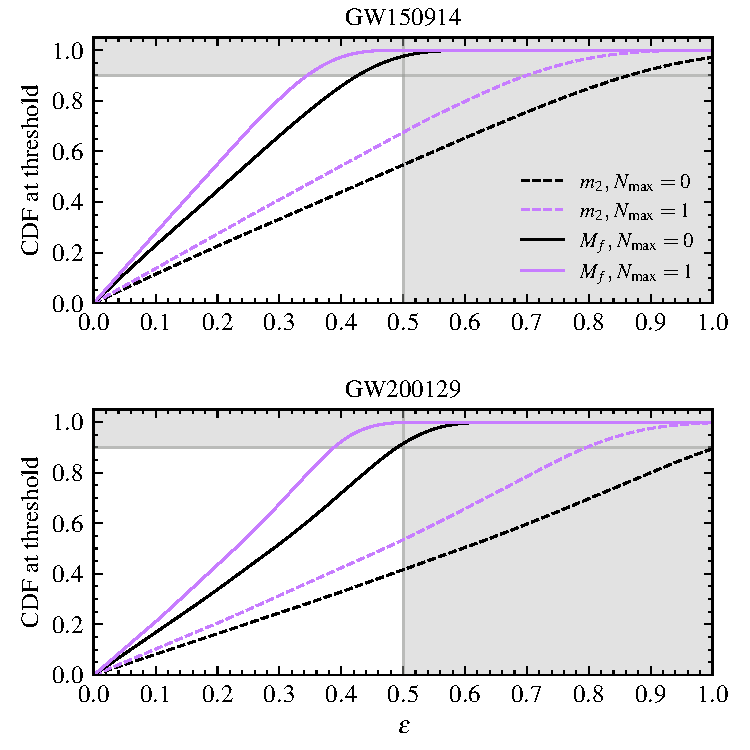
\includegraphics[width=\columnwidth]{figs/ceft_cdf_varying_threshold.pdf}
\caption{(Color online).~Similar to Fig.~\ref{fig:edgb_cdf}, but for the cubic EFT of GR.
We see that the CDF curves for $\gm = M_{f}$ are above 90\% for $\varepsilon =
1/2$ for both events, with and without including the $n = 1$ corrections to
the dominant QNM.
}
\label{fig:cEFT_cdf}
\end{figure}

\begin{table}[b]
\begin{tabular}{l l c c c}
\hline
\hline
$N_{\rm max}$ & Event & EFT    & ParSpec & Constraint ($\gm = M_{f}$) \\
              &       & bound? & bound?  &                            \\
\hline
  & GW150914  & Yes & Yes &  $\ell_{\rm cEFT} \leqslant 38.2$~km \\
0 & GW200129  & Yes & Yes &  $\ell_{\rm cEFT} \leqslant 42.5$~km \\
  & Combined  &     &     &  \cellcolor{black!10}$\ell_{\rm cEFT} \leqslant 38.2$~km \\
\hline
  & GW150914  & Yes  & No  &  -- \\
1 & GW200129  & Yes  & No  &  -- \\
  & Combined  &      &     &  -- \\
\hline
\hline
\end{tabular}
\caption{Detailed summary of our results the cubic EFT of GR for GW150914, GW200129, and
combined events using $\gm = M_{f}$, $\varepsilon = 1/2$ and quoting only 90\% credible results.
}
\label{tab:summary_ceft}
\end{table}

\subsection{Quartic Effective-Field-Theory of General Relativity}
\label{sec:results_qeft}

Let us now consider the quartic EFT of GR as our final example.
%
In Fig.~\ref{fig:qEFT_exec_sum} we show the posteriors on $\ell_{\rm qEFT}$ for GW150914 (top panel),
GW200129 (middle panel) for $N_{\rm max} = 0$, which are qualitatively similar to the cubic EFT of GR.
%
We find that both the EFT~\eqref{eq:eft_bound} and ParSpec~\eqref{eq:parspec_bound} are satisfied,
hence allowing us to infer bounds on $\ell_{\rm qEFT}$.
%
As Fig.~\ref{fig:qEFT_cdf} shows the CDFs for both events reach 90\% for $\gm = M_f$ before $\varepsilon = 1/2$.
%
Consequently, from the joint posterior of $\ell_{\rm qEFT}$ we quote our final result,
%
\begin{equation}
    \ell_{\rm qEFT} \leqslant 51.3~\textrm{km}\,.
\end{equation}

In this theory, we considered only $N_{\rm max} = 0$. We found that the
inclusion of the spin corrections yields waveforms which for $\ell_{\rm qEFT} \gtrsim 80$~km
for which the ringdown portions of the larger than the inspiral-plunge part \dots
%
To avoid this issue we lowered the value of $\ell^{\rm max}_{\rm qEFT}$, but by doing so we obtained posteriors
which were essentially uniform. Thus, we do not quote any results for $N_{\rm max} = 1$.
%
Table~\ref{tab:summary_qeft} summarizes our findings for the quartic EFT of GR.
%
\hs{Discuss. I don't have a good argument for why the $N_{\rm max} = 1$ simulations are breaking down other than
we just fail to compute the waveform for $\ell_{\rm qEFT} = 80~$~km for GW150914-like masses.}

\begin{figure}[t]
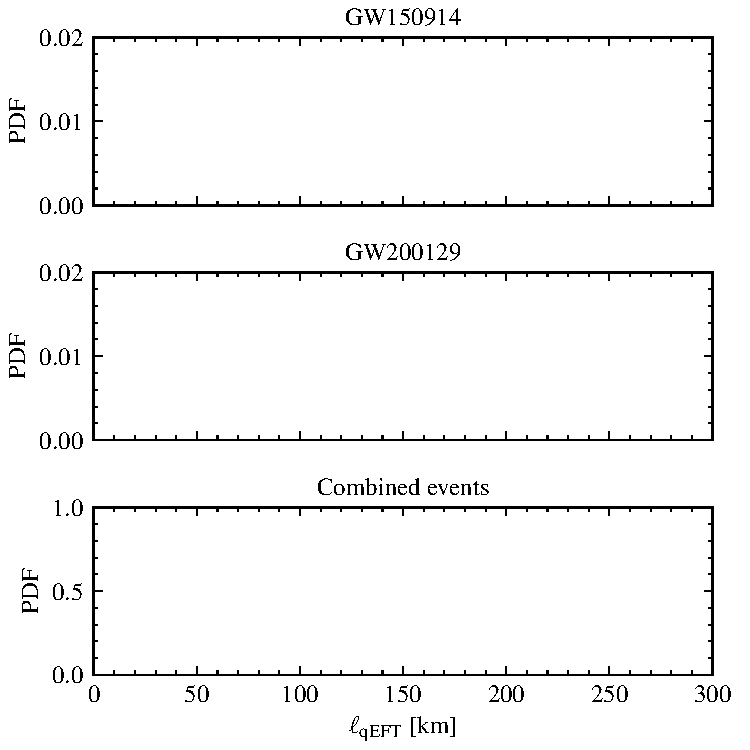
\includegraphics[width=\columnwidth]{figs/qeft_posteriors_combined.pdf}
\caption{(Color online).~Posterior distribution function for the coupling constant $\ell_{\rm qEFT}$ for
GW150914 (top panel), GW200129 (middle panel) and combined events (bottom panel).
}
\label{fig:qEFT_exec_sum}
\end{figure}

\begin{figure}[t]
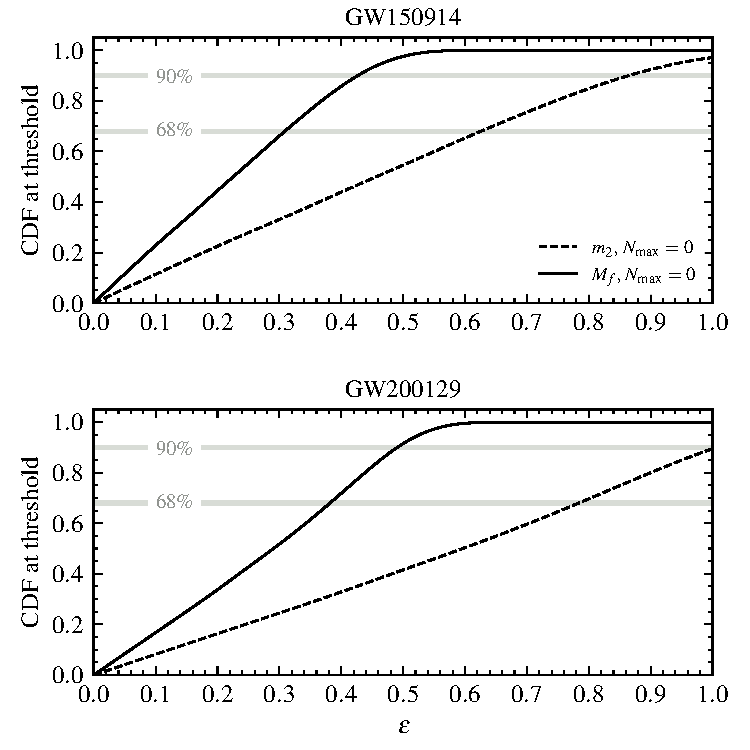
\includegraphics[width=\columnwidth]{figs/qeft_cdf_varying_threshold.pdf}
\caption{Similar to Fig.~\ref{fig:edgb_cdf}, but for the quartic EFT of GR.
We find that similarly to what happens in dCS gravity and the cubic EFT of GR, we
can place a constrain on $\ell_{\rm qEFT}$ when $\gm = M_f$ for both events at 90\% credibility.
}
\label{fig:qEFT_cdf}
\end{figure}

\begin{table}[h]
\begin{tabular}{l l c c c}
\hline
\hline
$N_{\rm max}$ & Event & EFT    & ParSpec & Constraint ($\gm = M_{f}$) \\
              &       & bound? & bound?  &                            \\
\hline
  & GW150914 & Yes & Yes  & $\ell_{\rm qEFT} \leqslant 51.7$~km \\
0 & GW200129 & Yes & Yes  & $\ell_{\rm qEFT} \leqslant 54.8$~km \\
  & Combined &     &      & \cellcolor{black!10}$\ell_{\rm qEFT} \leqslant 51.3$~km \\
% \hline
%   & GW150914 &  &     &    \\
% 1 & GW200129 &  &     &    \\
%   & Combined &  &     &    \\
\hline
\hline
\end{tabular}
\caption{Detailed summary of our results the quartic EFT of GR for GW150914, GW200129, and
combined events using $\gm = M_{f}$, $\varepsilon = 1/2$, and $N_{\rm max} = 0$. The quoted
result correspond to 90\% credible values.
}
\label{tab:summary_qeft}
\end{table}

% \begin{figure}[t]
% 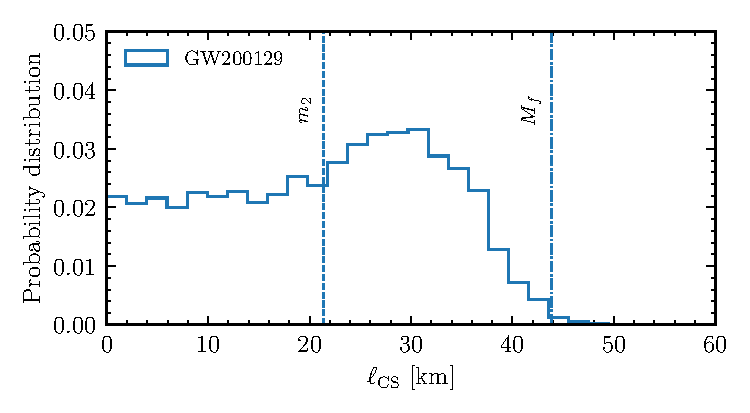
\includegraphics[width=\columnwidth]{figs/dcs_GW200129.pdf}
% \caption{Posterior probability distribution on $\ell_{\rm CS}$ with GW200129.
% The posterior shows that information was gained on this parameter relative to
% the initial uniform prior distribution $\ell_{\rm CS} \in [0,\, 200]$~km.
% %
% The vertical lines represent two threshold for the validity of the theory as
% an EFT.
% %
% The dotted line (labeled ``$m_2$'') at $\ell_{\rm CS} \approx 21.3$~km is
% given by the median value of the secondary's mass $\varepsilon \, (G m_2 / c^2)$.
% %
% The dot-dashed line (labeled ``$M_{f}$'') at $\ell_{\rm CS} \approx 43.8$~km is
% given by the median value of the remnant's mass $\varepsilon \, (G M_{f} / c^2)$.
% %
% For both, we used $\varepsilon = 0.5$.
% %
% If we take the latter as a length scale for the validity of dCS as an EFT, we
% have place upper bound on $\ell_{\rm CS} \leqslant 43.8$~km, within the
% approximation of our formalism.
% }
% \label{fig:dCS_bounds}
% \end{figure}
%
% \begin{figure}[t]
% 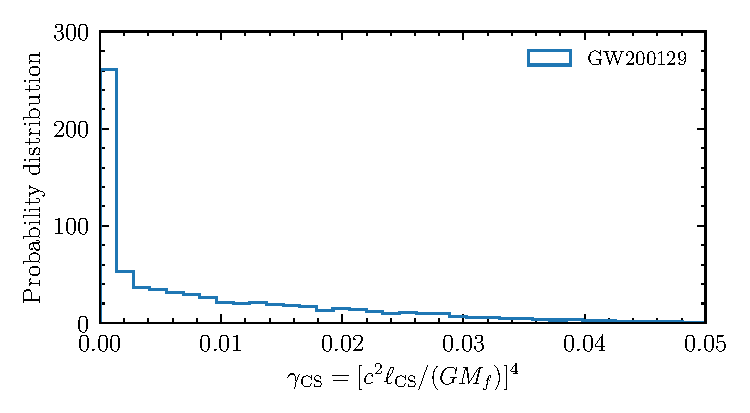
\includegraphics[width=\columnwidth]{figs/dcs_gamma_GW200129.pdf}
% \caption{Posterior probability distribution on $\gamma_{\rm CS}$ with GW200129.
% The posterior shows that the parameter $\gamma$ [see Eq.~\eqref{eq:def_gamma}]
% in dynamical Chern-Simons has a peak at zero, indicating consistency with GR.
% }
% \label{fig:dCS_gamma_plot}
% \end{figure}

%%%%%%%%%%%%%%%%%%%%%%%
\section{Conclusions}
\label{sec:conclusions}
%%%%%%%%%%%%%%%%%%%%%%%

% -------------------------------------------------------------
% \hs{Try to draw some conclusions that apply to all theories.}
% -------------------------------------------------------------

We presented an unified framework to combine the framework introduced
to model deviations to the GR QNMs~\cite{Maselli:2019mjd} with the \pSEOB~waveform model~\cite{Brito:2018rfr,Ghosh:2021mrv}.
%
We showed with concrete examples how theory-specific calculations QNM of
slowly-rotating BHs in modified gravity theories can be mapped onto the
theory-agnostic beyond-GR parameters of the ParSpec formalism.
%
Put together this allowed us to use the \pSEOB~waveform model to test four
modified gravity theories (EdGB, dCS, cubic, and quartic EFTs of GR) using
observational data from the GW events GW150914 and GW200129.
%
We found, in particular that, within the assumptions of our model and by
stacking posteriors, that the coupling constant of dCS gravity is bound to
$\ell_{\rm CS} \leqslant 34.5$~km.
%
In contrast, we could not place any constraint of the coupling constants in EdGB gravity $\ell_{\rm GB}$.
%
This dichotomy between these theories has an analogy with works that considered
the inspiral part of the GW signal alone.
%
In that case, it is dCS which is unconstrained, while EdGB, in principle can be
constrained, based on results for the closely related shift-symmetric version
of this theory.

Our work shows that there are theories of gravity (such as dCS) which can by-pass observational
constraints from the inspiral phase alone, {\it yet} would not, if we
analyze the ringdown.
%
We hope that our result thus serve as additional motivation for future work
modeling the late-inspiral, merger and ringdown of coalescing BHs in modified
gravity theories.

Let us discuss some avenues for future work \dots

\hs{TODO: say that we could try to expand the waveform model to include modification to
the inspiral part too; maybe through FTI~\cite{Mehta:2022pcn}?}

\hs{TODO: add that we could try to parametrize the final black hole mass and spin estimates formulas we
use at the moment~\cite{Hofmann:2016yih}. Maybe comment that a possible first attempt could follow~\cite{Buonanno:2007sv},
as done in~\cite{Jai-akson:2017ldo,Li:2020wse}. Say that ultimately we will need to informed by NR in beyond-GR.}

\hs{I suspect that by construction the $N_{\rm max} = 1$ cases will often fail to satisfy our
perturbative bounds. If so, add explanation here.}

% -----------------------------------------------------------------------------
% \hs{Say that the fact we spin correction look important reinforces the
% importance of calculation QNMs of spinning black holes beyond-GR.}
%
% \hs{Say it is important to go beyond mode calculation and actually understand
% how the QNM appear in the GW signal.}
% -----------------------------------------------------------------------------

% ------------------------------------------------------------------------------------
% HS: we fixed p in our work. We could leave it free in future studies study.
% This is similar to the 'number of dimensions'-like studies. Here it would
% tells us quite generically what is the dimension of the modification to the
% EH-action we include!
% ------------------------------------------------------------------------------------

\appendix

\section{Details of the determination of the theory-specific
ParSpec coefficients}
\label{app:map_details}

\subsection{Einstein-dilaton-Gauss-Bonnet}
\label{app:map_edgb}

\subsection{dynamical Chern-Simons}
\label{app:map_dcs}

% Let us show one concrete example of how this mapping is done.
%
In Ref.~\cite{Wagle:2021tam} the QNMs of slow-rotating BHs in dCS gravity were calculated
and it was found that the axial gravitational modes have their damping time increased as we
increase the Chern-Simons coupling $\ell_{\rm CS}$ at fixed spin $\chi$ of the BH.
%
Hence, according to the prescription of Sec.~\ref{sec:theory_specific_qnm}, this is the branch of QNMs we will select.

We can now proceed to determine $\delta\omega^{(n)}$ and $\delta\tau^{(n)}$ as follows.
%
Using the fitting formula Eq.~(54a) of~\cite{Wagle:2021tam}, namely,
%
\begin{equation}
    M \omega_{\rm CS} = c_{1} + c_{2} \kappa \zeta + (c_{3} + c_{4} \kappa \zeta) \, (1 - \chi)^{c_{5} + c_{6} \kappa \zeta},
    \label{eq:omega_dsc_eg}
\end{equation}
%
and similarly for the imaginary part ${\rm Im}(\sigma_{\rm CS}) =  - 1 / \tau_{\rm CS}$.
%
Here $\kappa = 1/(16 \pi)$, $\zeta = \ell_{\rm CS}^{4} / (M^4 \kappa)$, and thus
%
\begin{equation}
\kappa \zeta = (\ell_{\rm CS} / M)^4 \,,
\end{equation}
%
and $c_{i}$ are fitting coefficients which can be found in Ref.~\cite{Wagle:2021tam}, Table II.
%
In the context of a binary BH merger, $M$ is interpreted as the remnant mass $\Mf$.

We now expand Eq.~\eqref{eq:omega_dsc_eg} to leading-orders in $\chi$ and $\ell_{\rm CS}$, and
gather the terms proportional to $\ell_{\rm CS}$.
%
We obtain
%
\begin{align}
    \Mf \, \omega_{\rm CS} &=
    \left[ 0.3722 + 1.1945 (\ell_{\rm CS} / \Mf)^4 \right]
    \nonumber \\
    &\quad + \left[0.1861 + 5.1828 (\ell_{\rm CS} / \Mf)^4 \right] \, \chi\,,
    \label{eq:omega_dcs_interm}
\end{align}
%
where we made use of the numerical value of the coefficients $c_{i}$.
%
We find that (reassuringly) that the nonrotating GR part of the expression above agree with $\omega^{(0)}$ of Ref.~\cite{Maselli:2019mjd}
to 0.5\% relative percent error. The same error estimate is larger ($\approx 20$\%) for the linear-in-spin coefficient;
0.1861 in comparison to 0.1258 of Ref.~\cite{Maselli:2019mjd}.
%
We attribute this difference to Ref.~\cite{Wagle:2021tam} having fitted Eq.~\eqref{eq:omega_dsc_eg} to QNM data compute to linear-order in spin, whereas~\cite{Maselli:2019mjd}
fitted Eq.~\eqref{eq:kerr_expansion} to Kerr QNM valid to all orders in spin.

We can now isolate the dCS corrections from Eq.~\eqref{eq:omega_dcs_interm} and
compare against Eq.~\eqref{eq:qnm_nongr_iso}, to find
%
\begin{equation}
p_{\rm CS} = 4\,, \quad \delta \omega^{(0)}_{\rm CS} = 3.1964\,, \quad \delta \omega^{(1)}_{\rm CS} = 41.199\,.
\label{eq:cs_omega_coefs}
\end{equation}

We can carry the same steps for $\tau_{\rm CS}$ and find
%
\begin{equation}
\delta \tau^{(0)}_{\rm CS} = 6.3619\,, \quad \delta \tau^{(1)}_{\rm CS} = 794.66\,.
\label{eq:cs_tau_coefs}
\end{equation}
%
which completes the set of fixed parameters beyond-GR parameters in the ringdown of the \pSEOB{} waveform model.
%
We remark that the alarmingly large values of $\delta \omega_{\rm CS}^{(1)}$ and $\delta \tau_{\rm CS}^{(1)}$
are compensated by the assumptions that $(\ell_{\rm CS} / M_f)^2$ and $\chi$ are much less than unity. These
are the assumptions used to calculate the QNM frequencies in Ref.~\cite{Wagle:2021tam}.

\subsection{Effective-field-theories GR}
\label{app:map_eftofgr}



%%%%%%%%%%%%%%%%%
\section*{Acknowledgements}
\label{sec:acknowledgements}
%
We thank Emanuele Berti, Andrea Maselli, Caio F. B. Macedo, Deyan Mihaylov,
Serguei Ossokine, Scott E. Perkins, and Helvi Witek for discussions.
%
We are grateful for the computational resources provided by the Max Planck
Institute for Gravitational Physics in Potsdam, specifically the
high-performace computing cluster Hypatia and to Steffen Grunewald for
assistance.
%
The authors would like to thank everyone at the frontline of the Covid-19
pandemic.
%%%%%%%%%%%%%%%%%

% \bibliographystyle{apsrev}
\bibliography{paper_alt_theor_bounds}

\end{document}
